\documentclass[xcolor=dvipsnames]{beamer}
\usepackage[T1]{fontenc}
\usepackage[utf8]{inputenc}
\usepackage[english,slovak]{babel}

\usepackage{amsmath}
\usepackage{amsthm}
\usetheme{Pittsburgh}
\useoutertheme{shadow}

\usepackage{graphicx}
\usepackage{caption}
\usepackage{subcaption}

\usepackage[]{algorithm2e}
\usepackage{listings}
 \setbeamercovered{transparent}
 \usepackage{cuted}
\usepackage[export]{adjustbox}
\usepackage{mathtools}

\usepackage{lipsum}

\newcommand\Wider[2][3em]{%
\makebox[\linewidth][c]{%
  \begin{minipage}{\dimexpr\textwidth+#1\relax}
  \raggedright#2
  \end{minipage}%
  }%
}

%-------------------------------------------------------------------------------------
\title{\bf Reinforcement learning}
\author{Michal CHOVANEC, PhD.}


%\setbeamertemplate{footline}[frame number]{}
\setbeamertemplate{navigation symbols}{}


\date[EURP]{\it March 2018}
\begin{document}

\begin{frame}
\titlepage
\centering{Fakulta riadenia a informatiky}
\end{frame}


\begin{frame}{\bf Problem definition}
\begin{itemize}
 \item learn to play game with unknow rules
 \item input  : state and reward
 \item output : action and total score
 \item $Q(s, a)$ : learn Q function
\end{itemize}
\centering

{\color{red} \bf agent never sees required value (required action)}


\begin{figure}
\centering
\begin{minipage}{.5\textwidth}
  \centering
  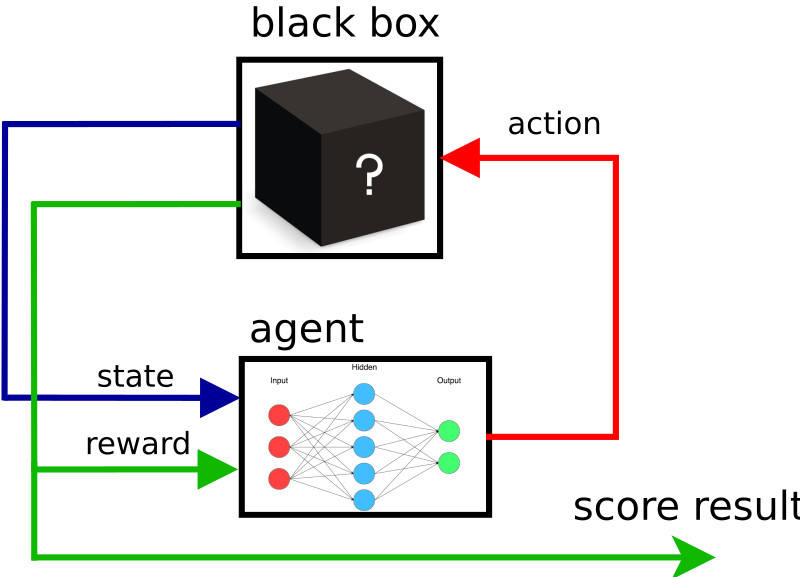
\includegraphics[scale=0.2]{../../diagrams/rl_mechanism.jpg}
\end{minipage}%
\begin{minipage}{.5\textwidth}
  \centering
  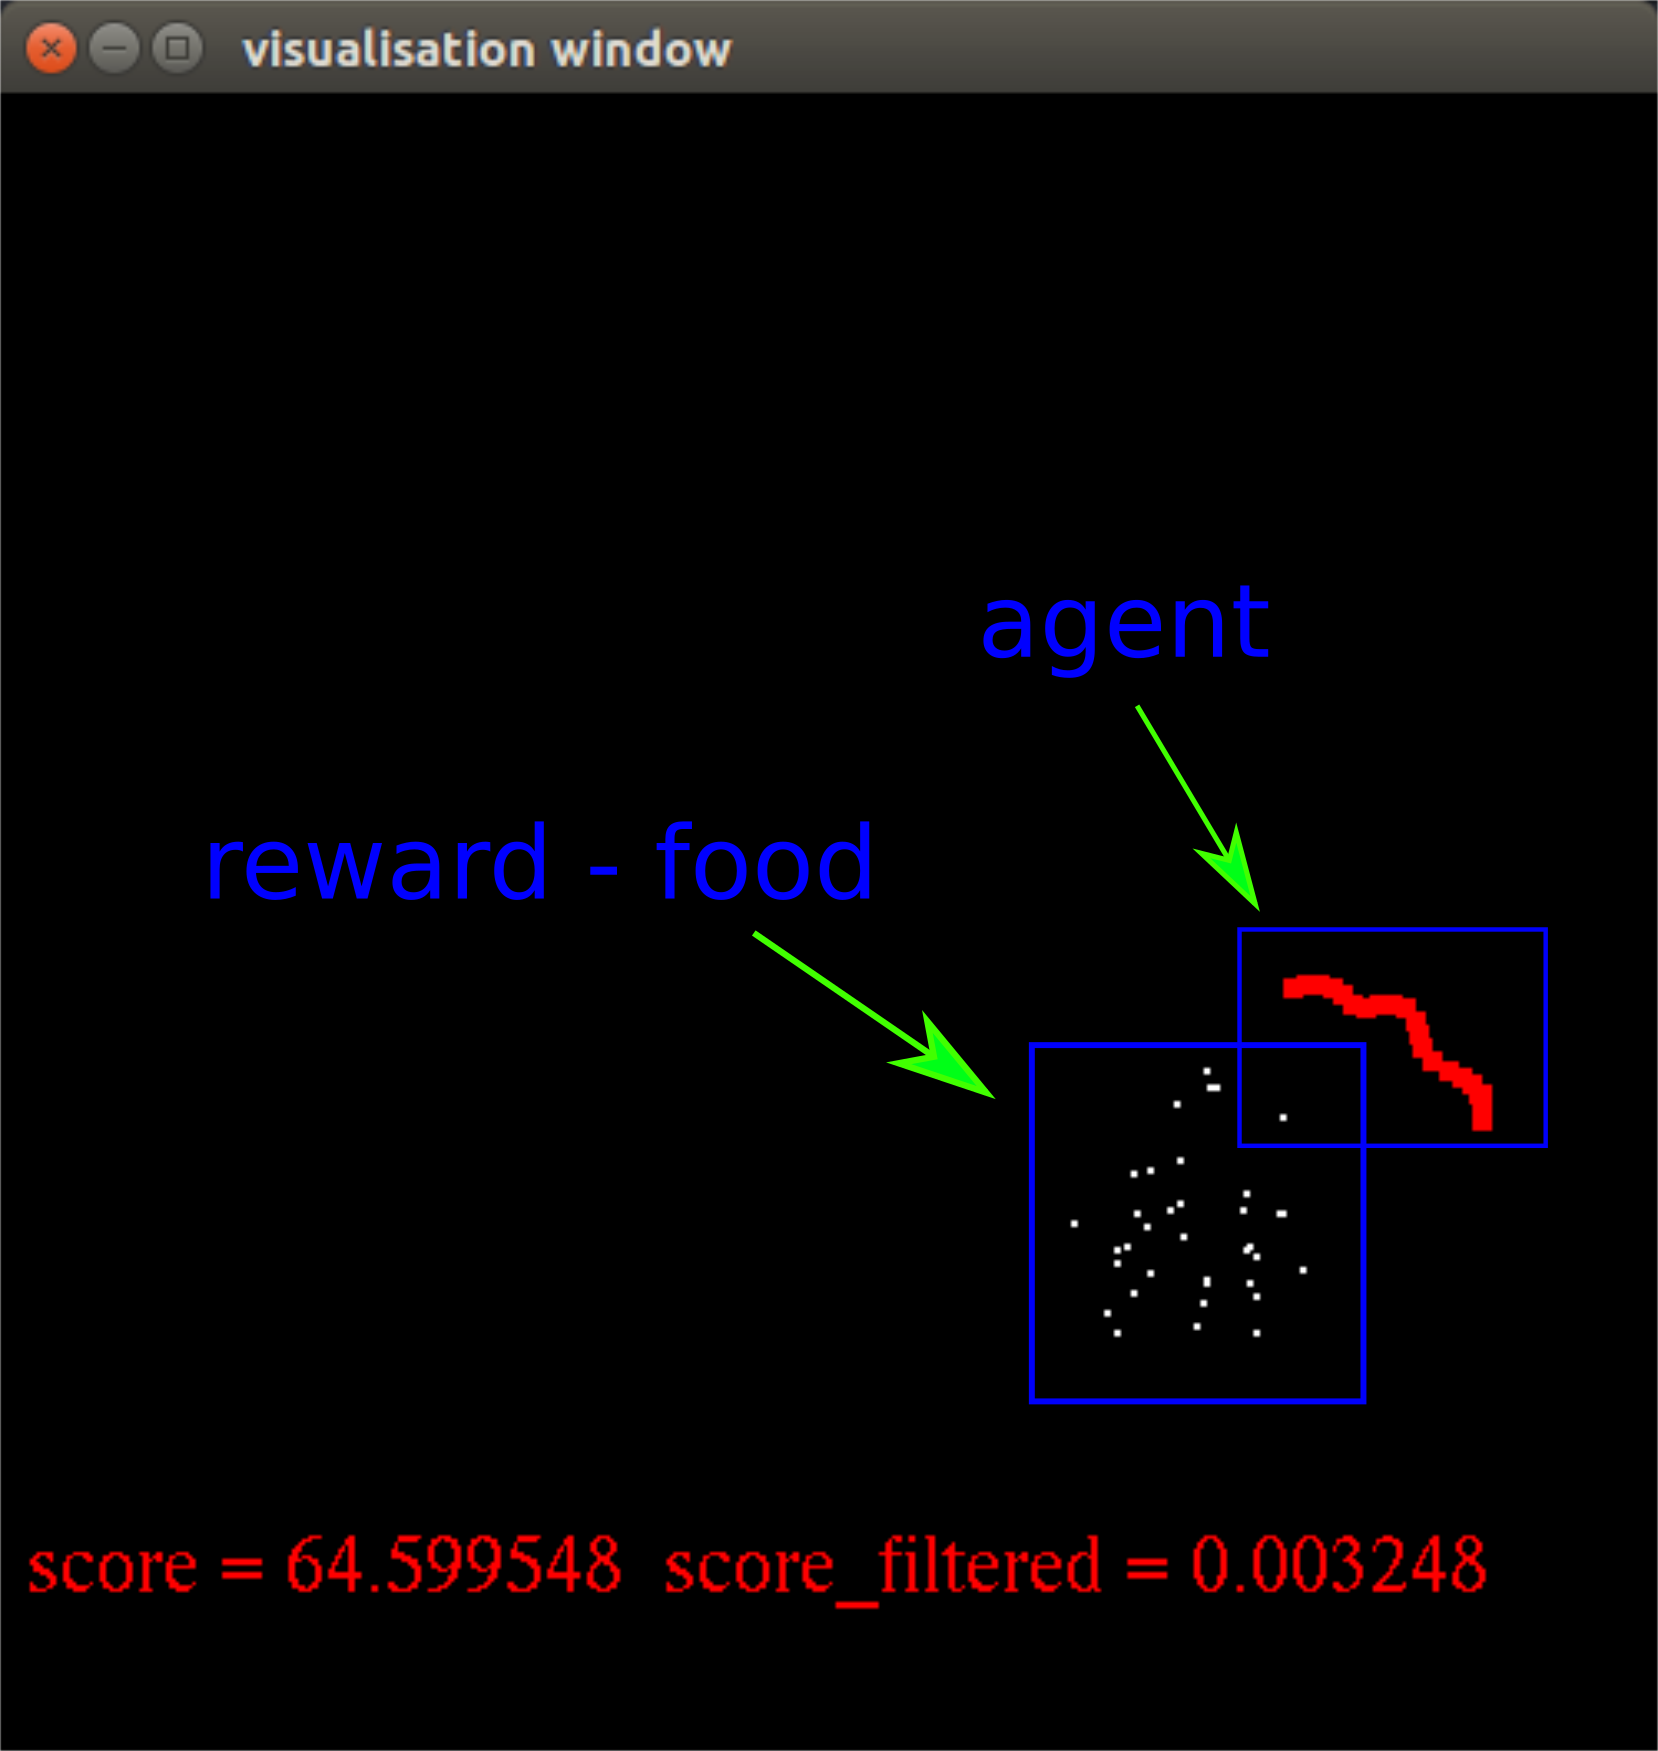
\includegraphics[scale=0.2]{../../diagrams/worms_rl_game_desc.png}
\end{minipage}
\end{figure}



\end{frame}


\begin{frame}{\bf Q-learning algorithm}
\begin{align*}
Q'(s, a) = R(s, a) + \gamma \max_{a' \in A}Q(s', a')
\end{align*}
where \\
$Q(s, a)$ is previous state \\
$Q(s', a')$ is actual state \\
$R(s, a)$ is reward obtained in state $s$ after executing action $a$ \\
$\gamma$ is discount factor $\gamma \in \langle0, 1\rangle$ \\
\begin{figure}[htbp]
  \centering
  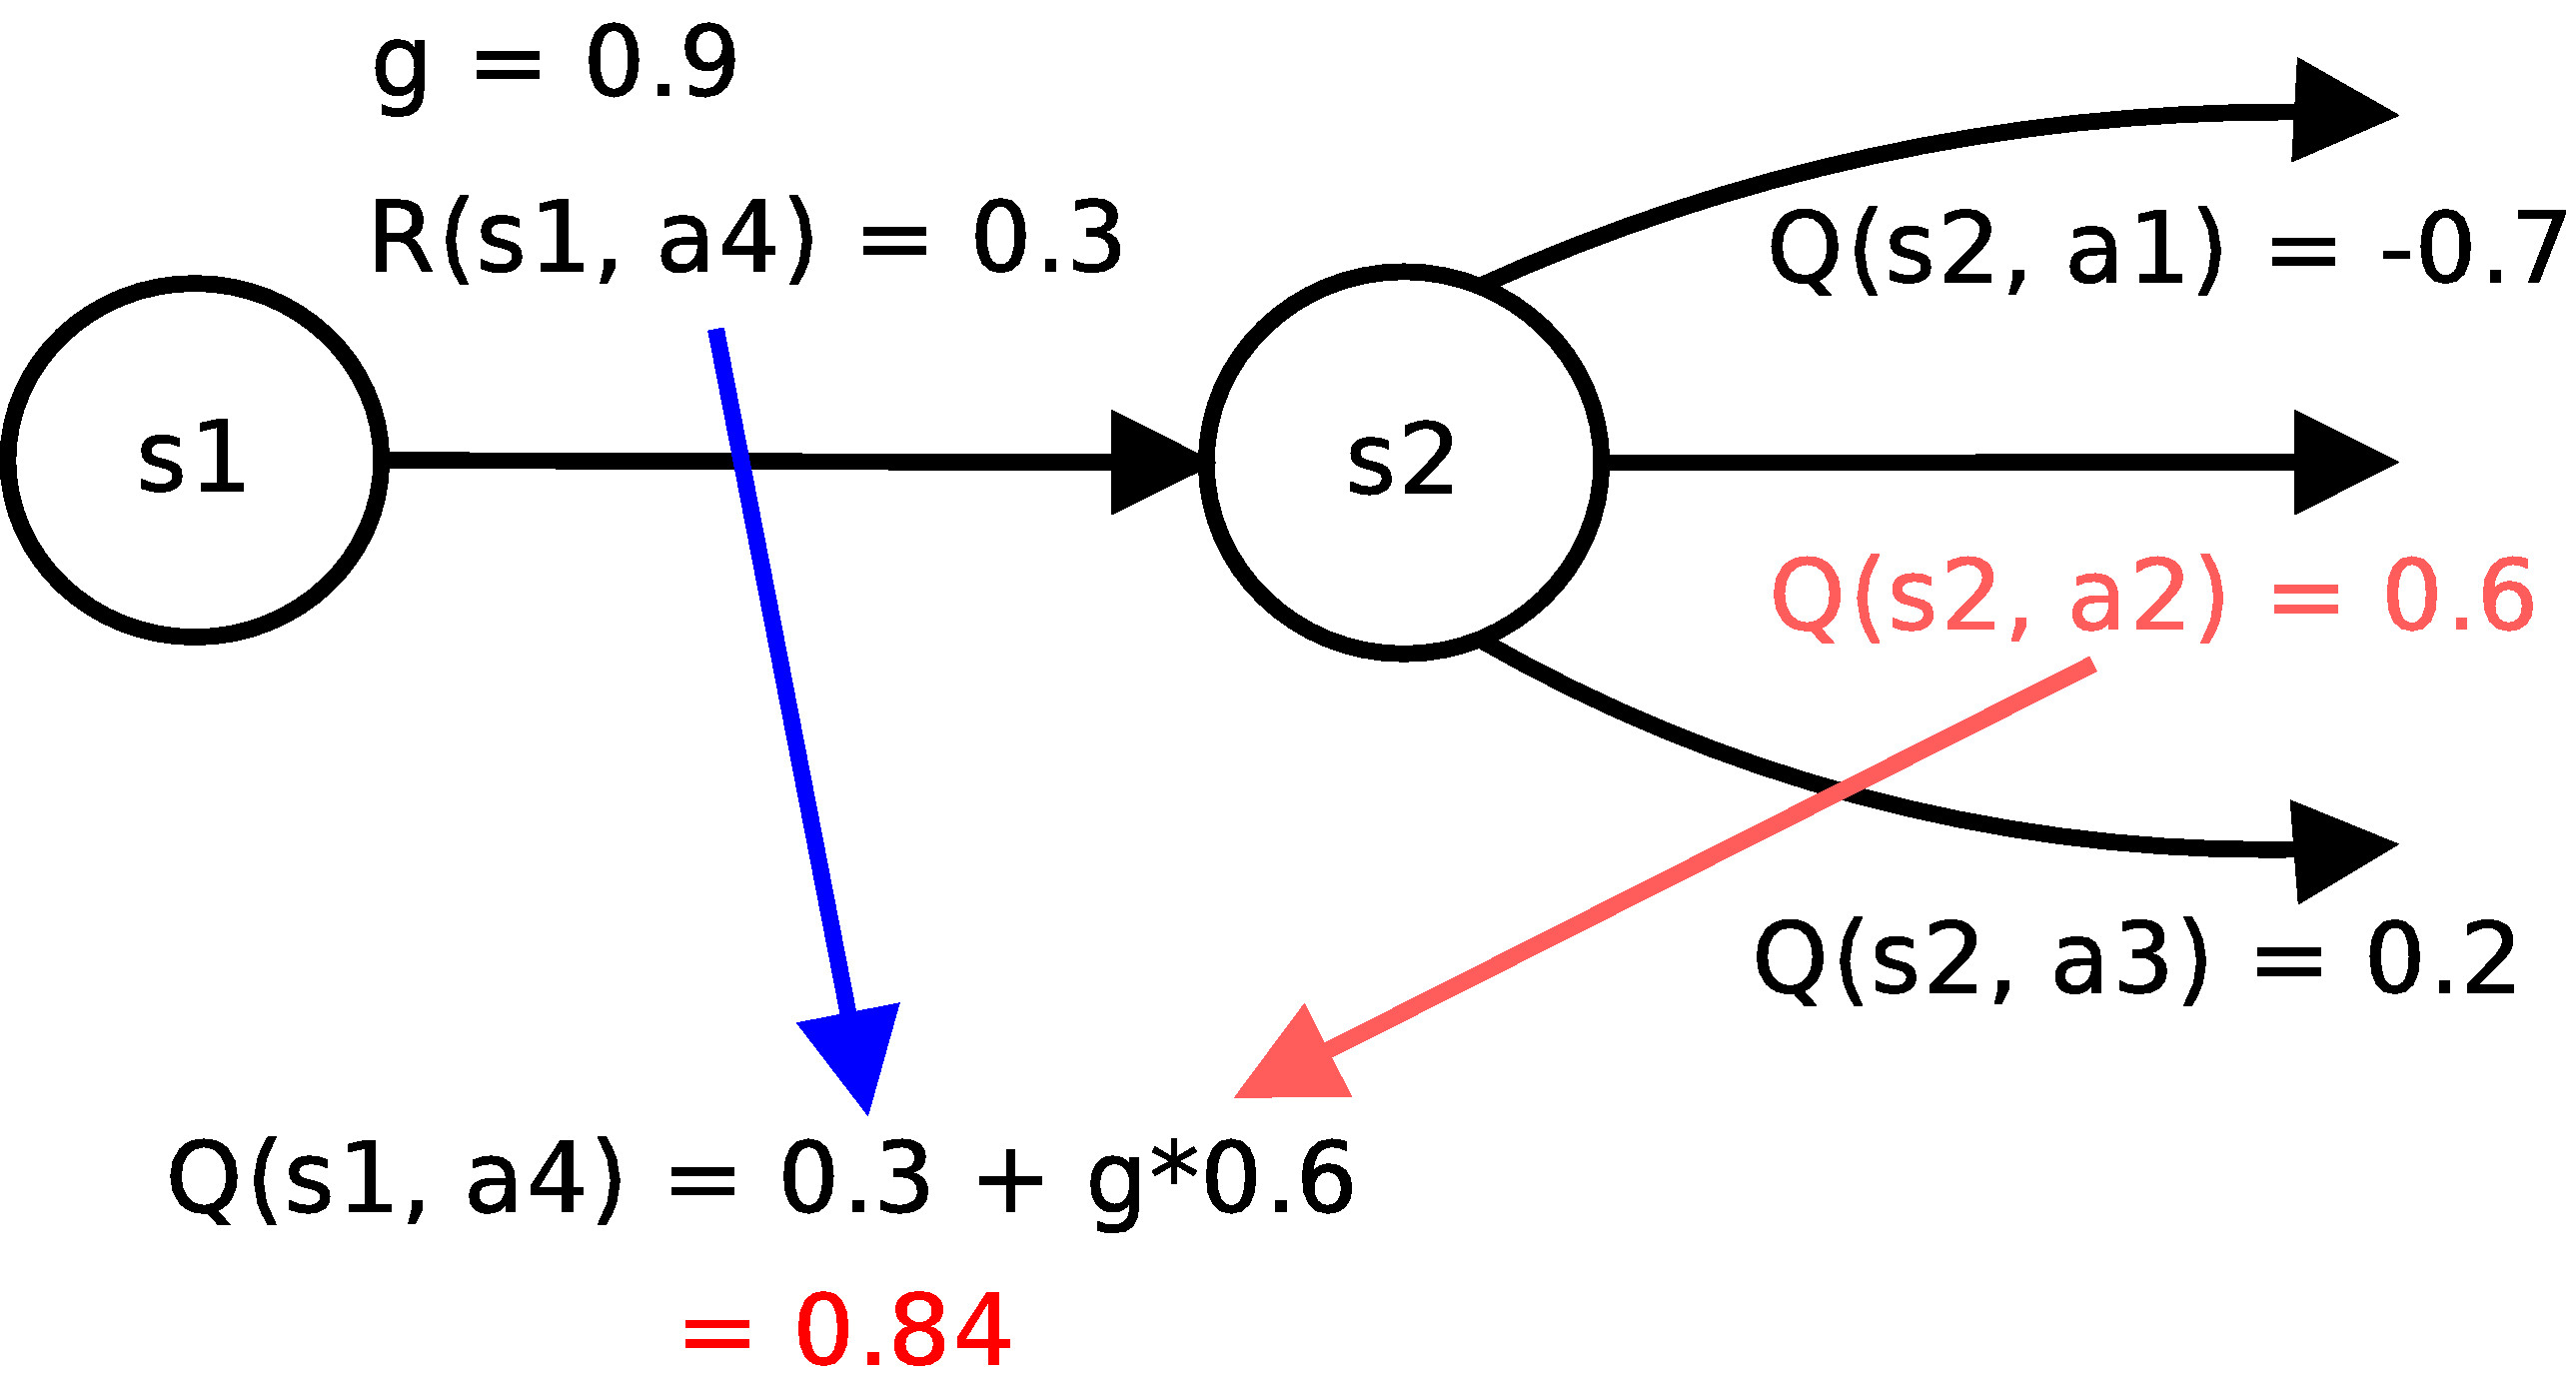
\includegraphics[scale=0.3]{../../diagrams/q_learning_detail.jpg}
\end{figure}



\end{frame}


\begin{frame}{\bf SARSA algorithm}
State Action Reward State Action
\begin{align*}
Q'(s, a) = (1-\alpha)Q(s, a) + \alpha(R(s, a) + \gamma Q(s', a'))
\end{align*}
where \\
$Q(s, a)$ is previous state \\
$Q(s', a')$ is actual state \\
$R(s, a)$ is reward obtained in state $s$ after executing action $a$ \\
$\gamma$ is discount factor $\gamma \in \langle0, 1\rangle$ \\
$\alpha$ is learning rate $\alpha \in (0, 1)$
\begin{figure}[htbp]
  \centering
  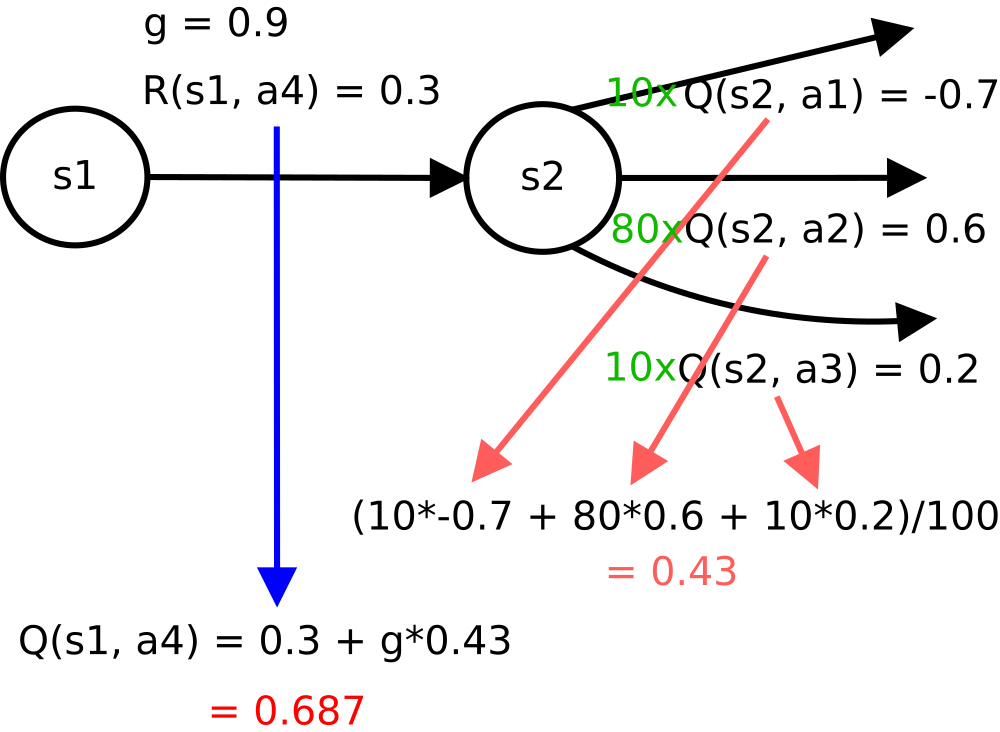
\includegraphics[scale=0.17]{../../diagrams/sarsa_learning_detail.png}
\end{figure}


\end{frame}


\begin{frame}{\bf Storing Q values}

\begin{itemize}
 \item table
 \item linear combination of basis function (handmade features)
 \item Kenerva's sparse encoding
 \item neural network
\end{itemize}

problems
\begin{itemize}
 \item state correlations
 \item nonstationary Q values
 \item convergence to optimal strategy
\end{itemize}

\end{frame}


\begin{frame}{\bf Neural network approximator - deep reinforcement learning}

\begin{figure}[htbp]
  \centering
  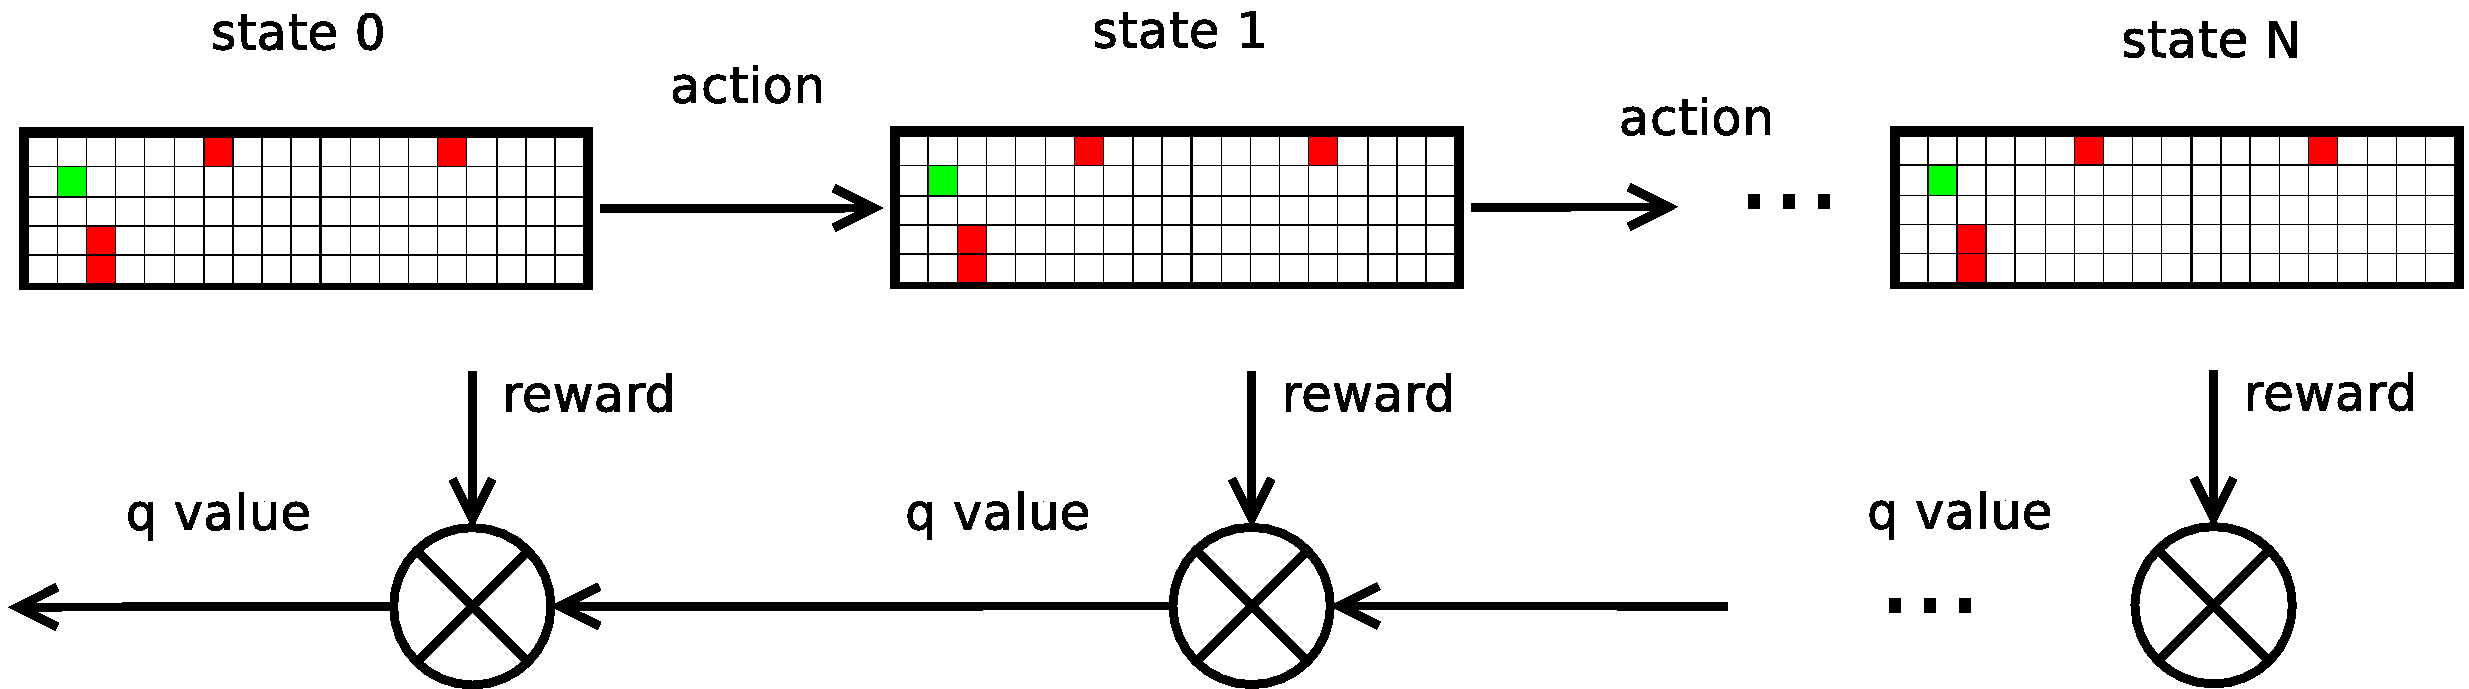
\includegraphics[scale=0.3]{../../diagrams/rl_nn_learn.png}
\end{figure}


\begin{figure}[htbp]
  \centering
  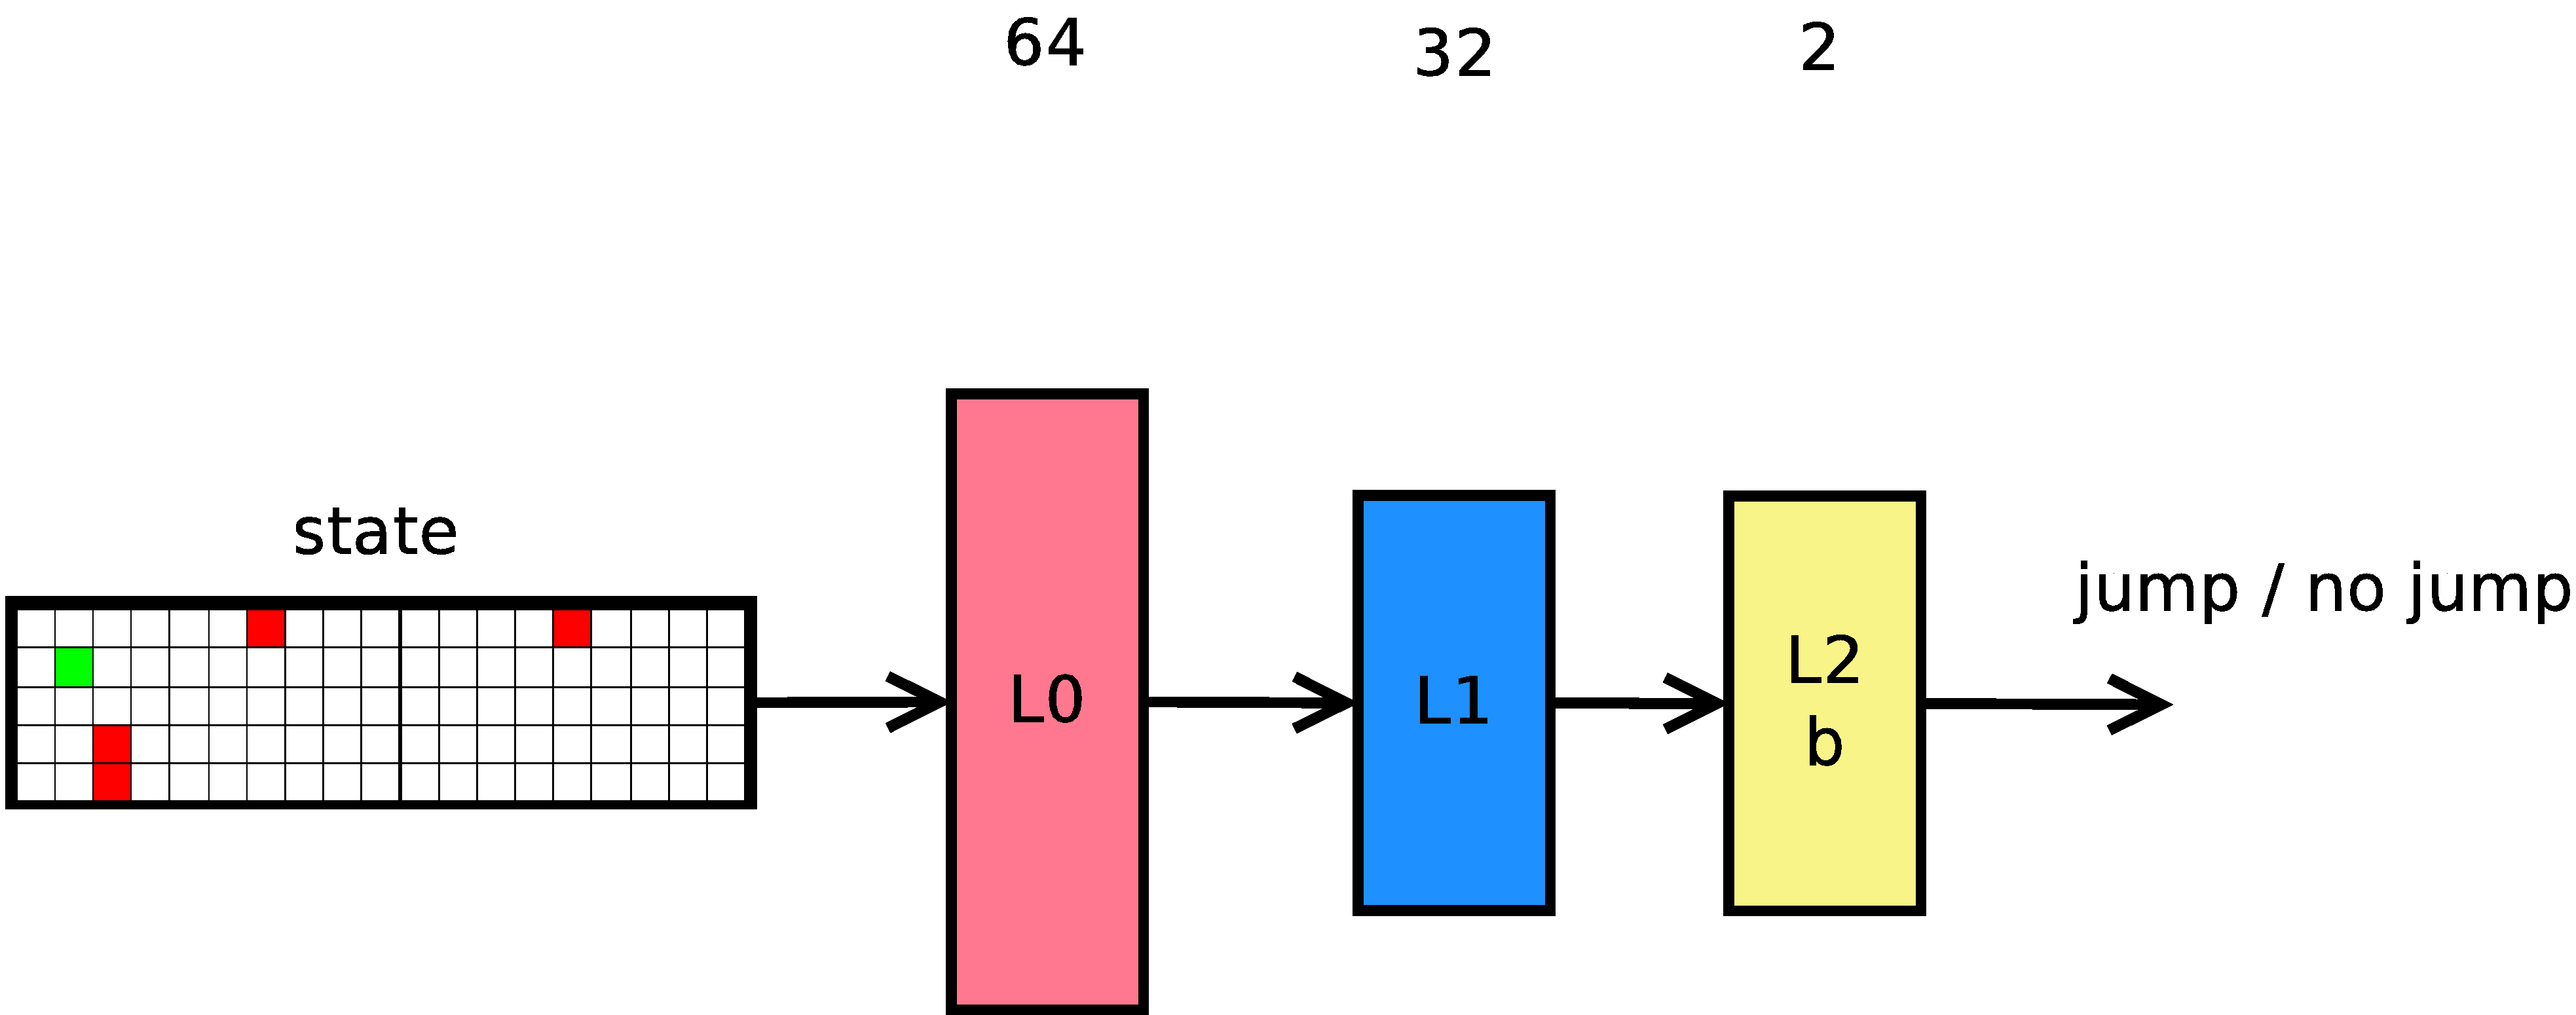
\includegraphics[scale=0.3]{../../diagrams/fnn.png}
\end{figure}

\end{frame}



\begin{frame}{\bf Speed up learning}

\begin{figure}[htbp]
  \centering
  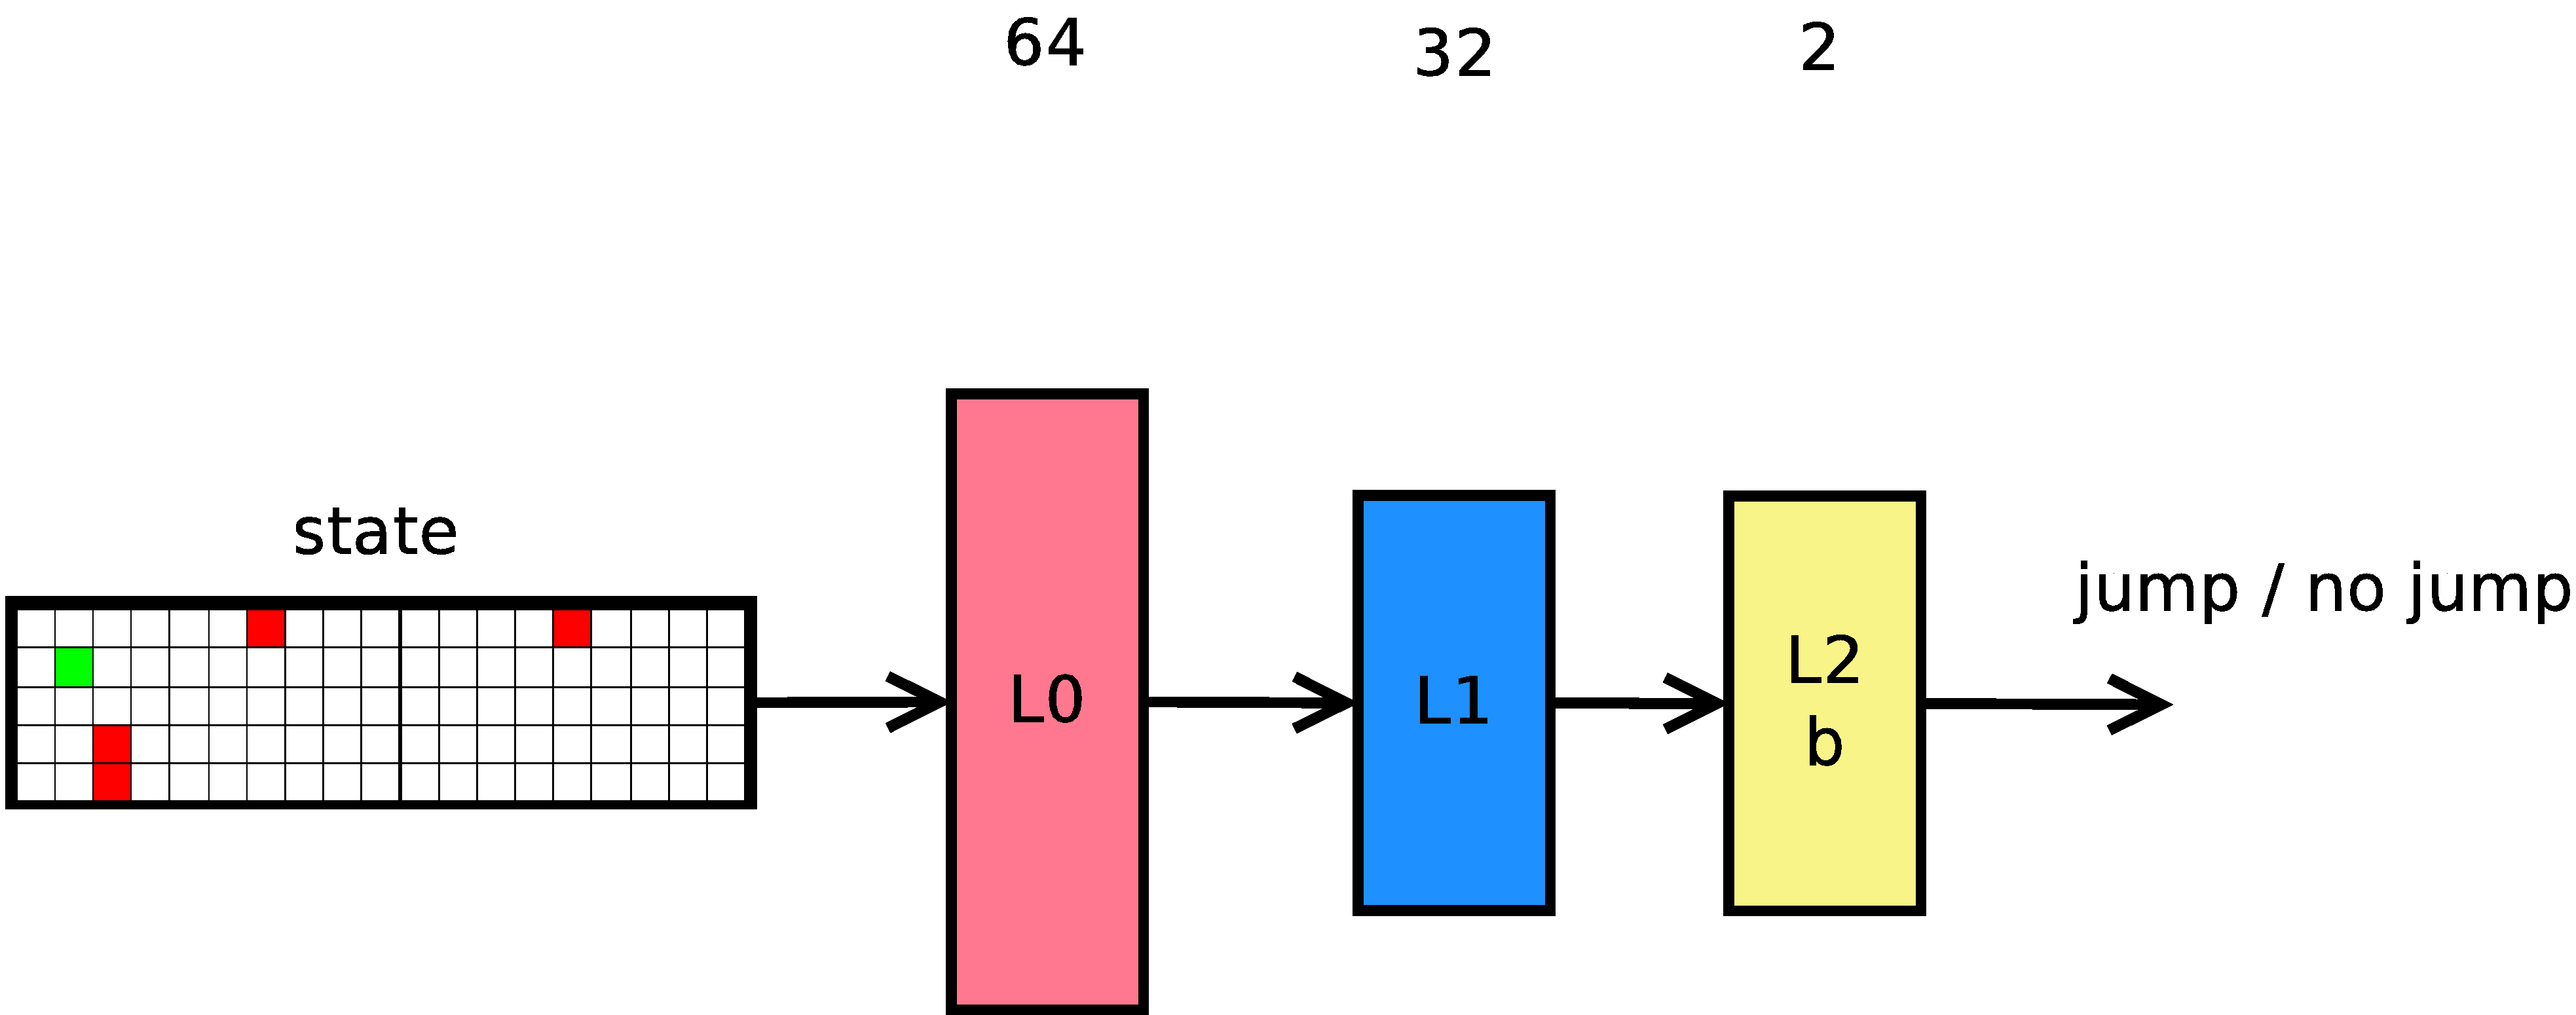
\includegraphics[scale=0.21]{../../diagrams/fnn.png}
  \caption*{common feed forward neural network}
\end{figure}

\begin{figure}[htbp]
  \centering
  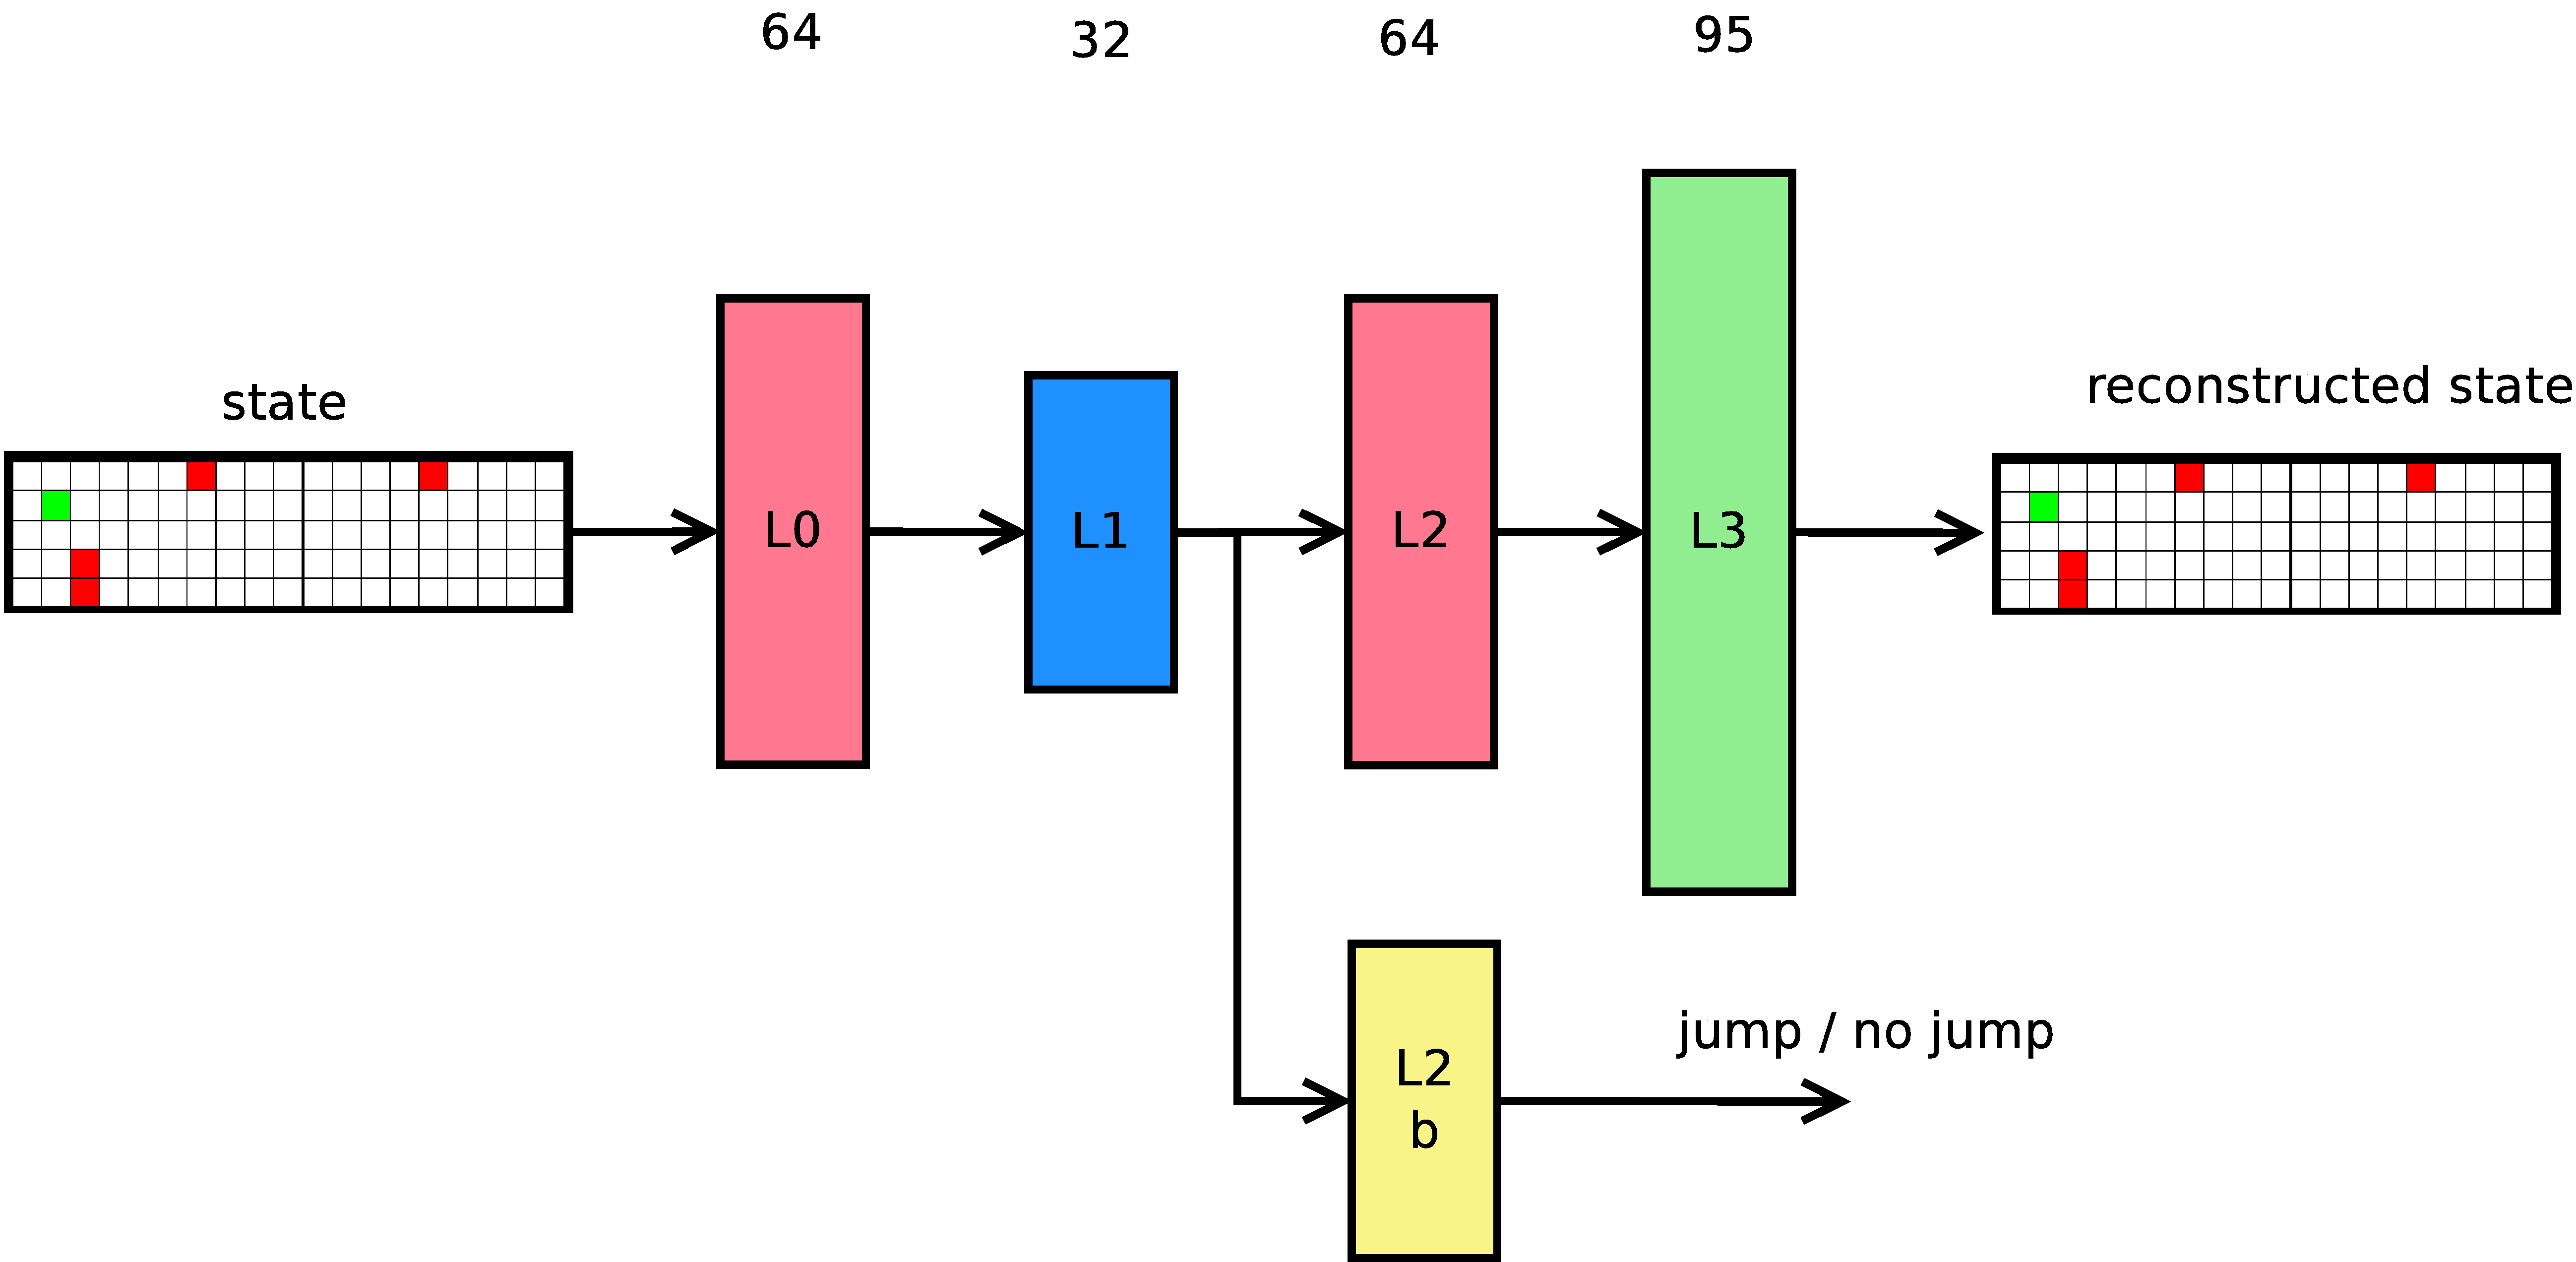
\includegraphics[scale=0.21]{../../diagrams/hnn.png}
  \caption*{stacked autoencoder + feed forward neural network}
\end{figure}

\end{frame}


\begin{frame}{\bf Sparse weights}

\begin{equation*}
  \label{eq:weights_training}
  \Delta w = \eta E x \frac{df(y)}{dw} - \lambda sgn(w)
\end{equation*}

where \\
$E$ is error, \\
$x$ is input, \\
$y$ is output, \\
$f$ is activation function (ReLU, tanh, softmax ...), \\
$\eta$ is learning rate , \\
$\lambda$ is sparsity parameter

\end{frame}



\begin{frame}{\bf Arcade game experiment}


\begin{figure}[htbp]
  \centering
  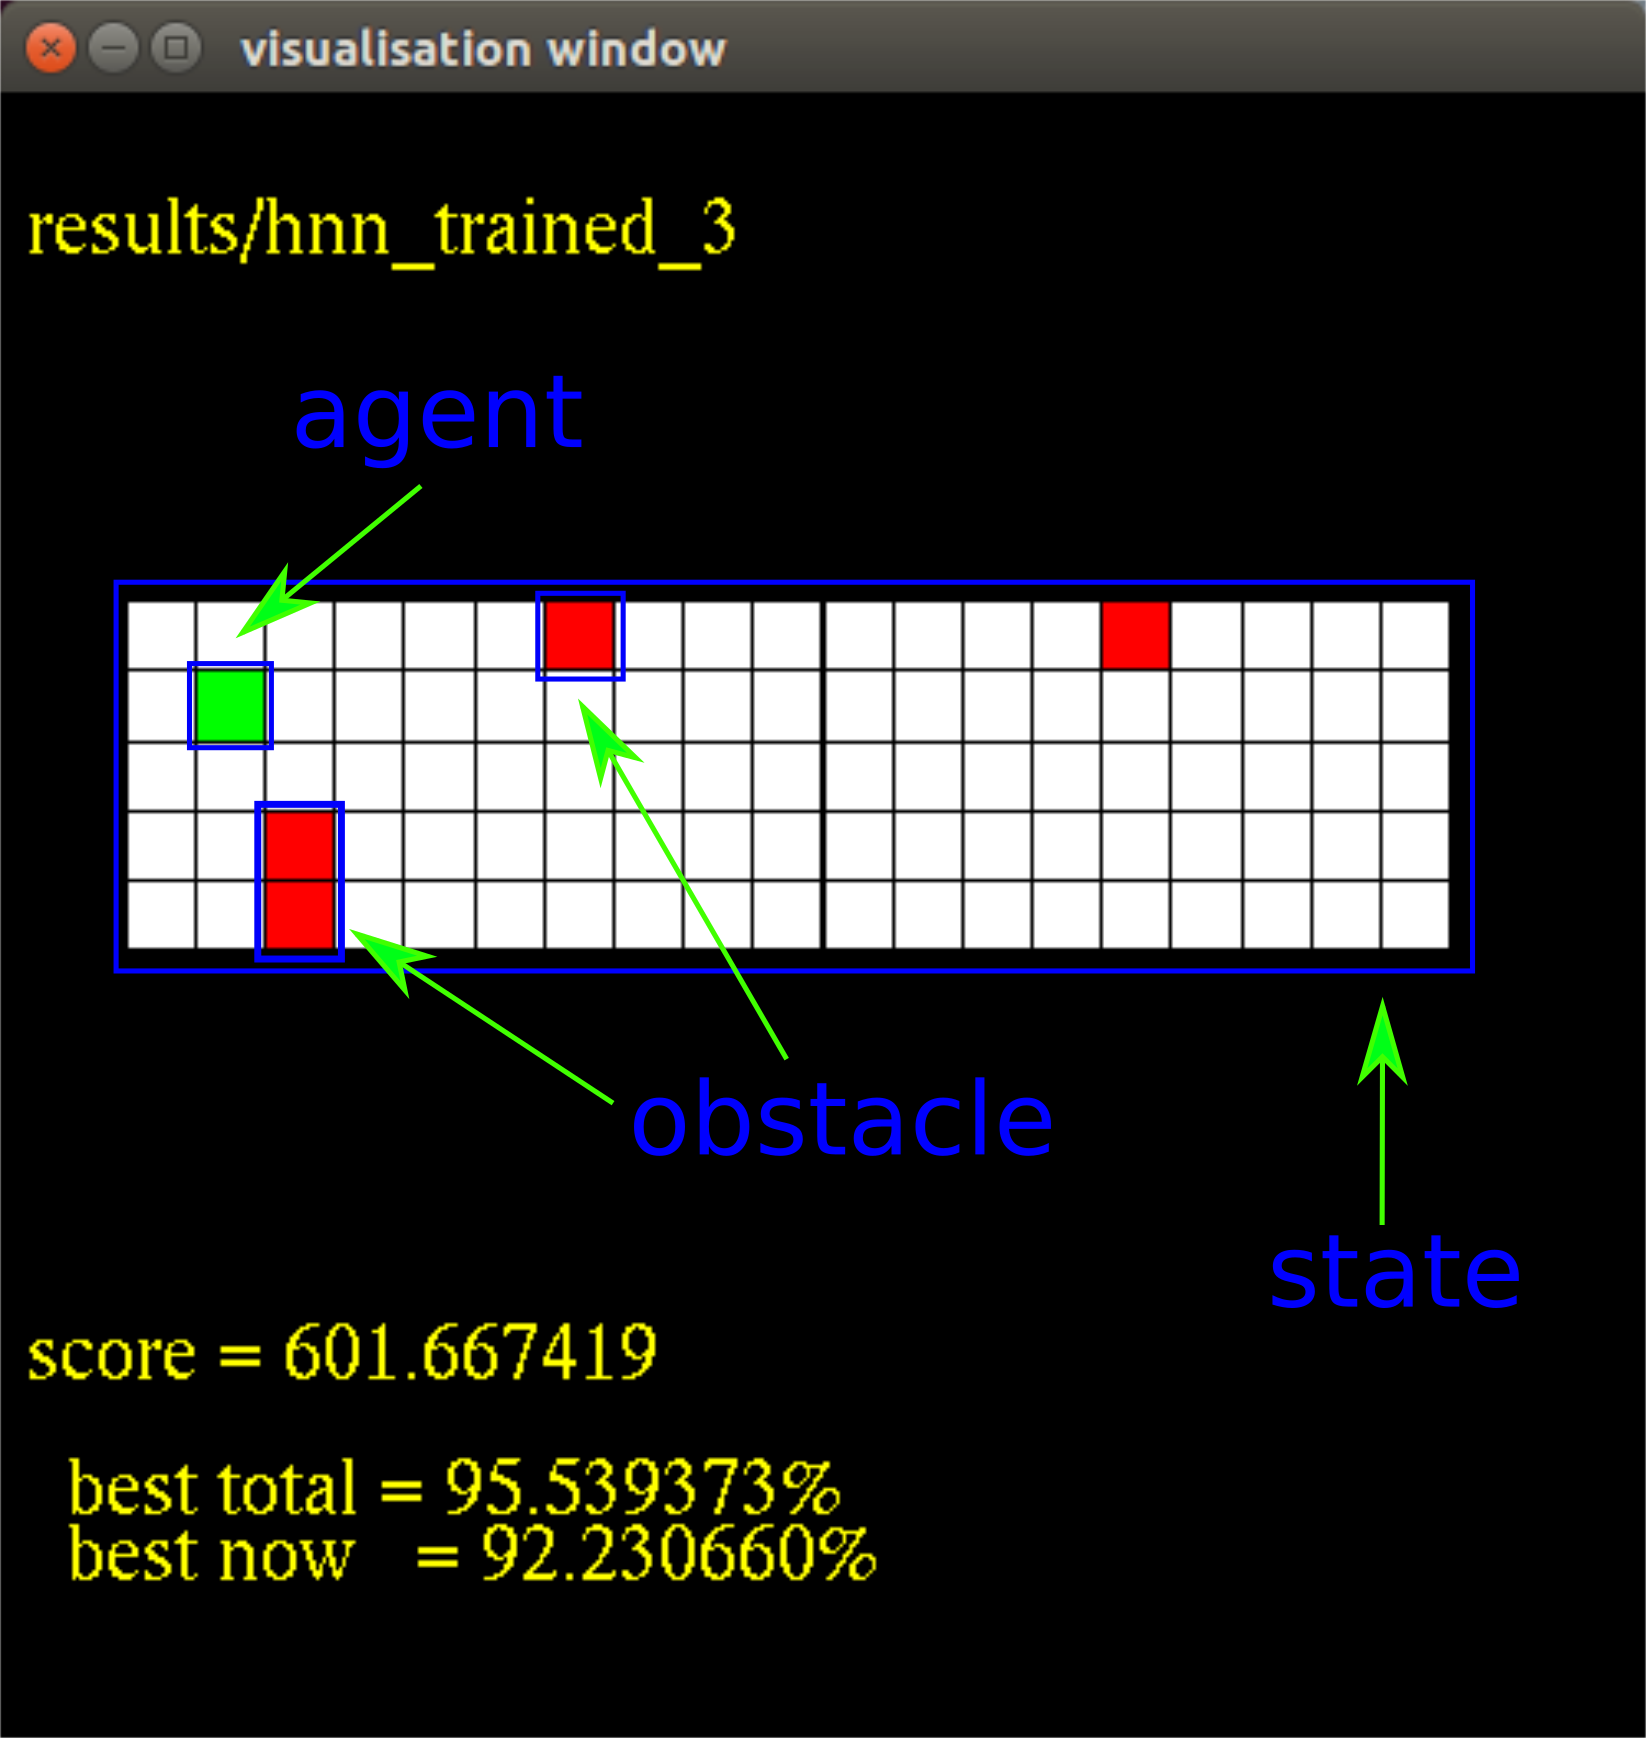
\includegraphics[scale=0.21]{../../diagrams/arcade_rl_game_desc.png}
\end{figure}

{
\tiny

\begin{table}[!h]
\centering
\begin{tabular}{|l|l|l|l|l|}
\hline
                        & FNN sparse & FNN no sparse & AE+FNN  sparse & AE+FNN no sparse \\ \hline
unsupervised iterations & 0          & 0             & 100000         & 100000           \\ \hline
supervised iterations   & 200000     & 200000        & 200000         & 200000           \\ \hline
iterations per slice    & 0          & 0             & 50000          & 50000            \\ \hline
learning rate           & 0.0005     & 0.0005        & 0.0005         & 0.0005           \\ \hline
init weight range       & 0.1        & 0.1           & 0.1            & 0.1              \\ \hline
dropout                 & 0          & 0             & 0              & 0                \\ \hline
lambda                  & 0.00000001 & 0             & 0.00000001     & 0                \\ \hline
\end{tabular}
\end{table}

}

\end{frame}


\begin{frame}{\bf Sparsity results}

\begin{figure}[!htb]
\centering
\begin{minipage}{.5\textwidth}
  \centering
  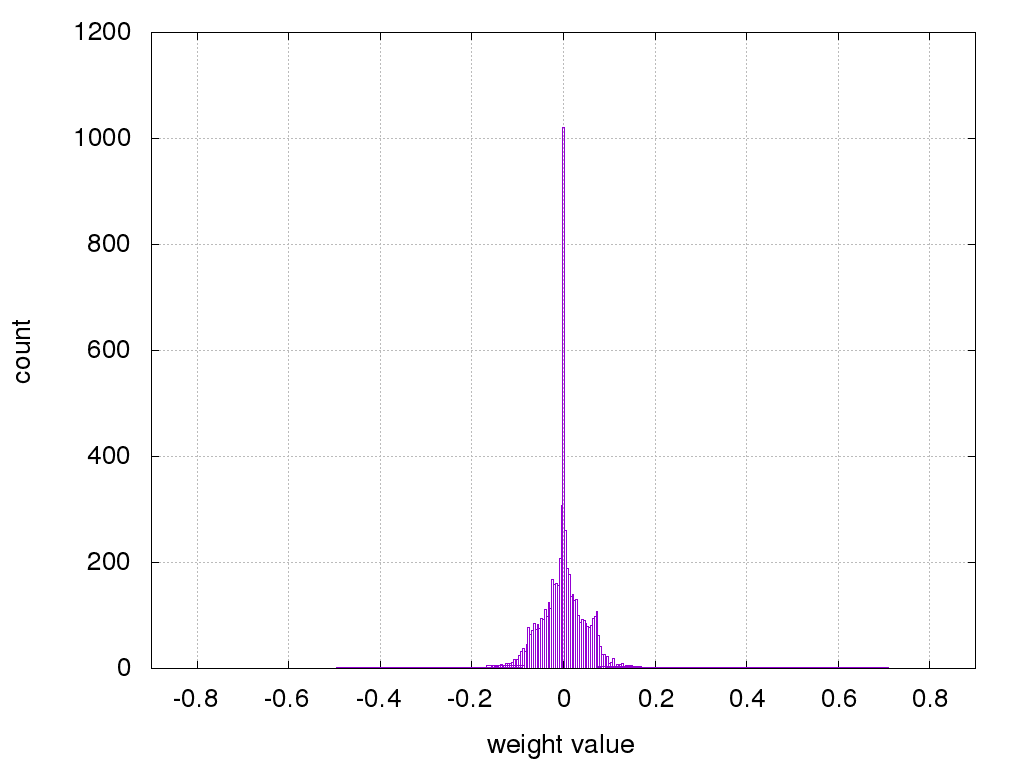
\includegraphics[scale=0.15]{../../results/rl_arcade/fnn_trained_0/supervised/layer_1_histogram.png}
  \captionof*{figure}{\tiny FNN sparse weights histogram}
  \label{img:FNN sparse weights histogram}
\end{minipage}%
\begin{minipage}{.5\textwidth}
  \centering
  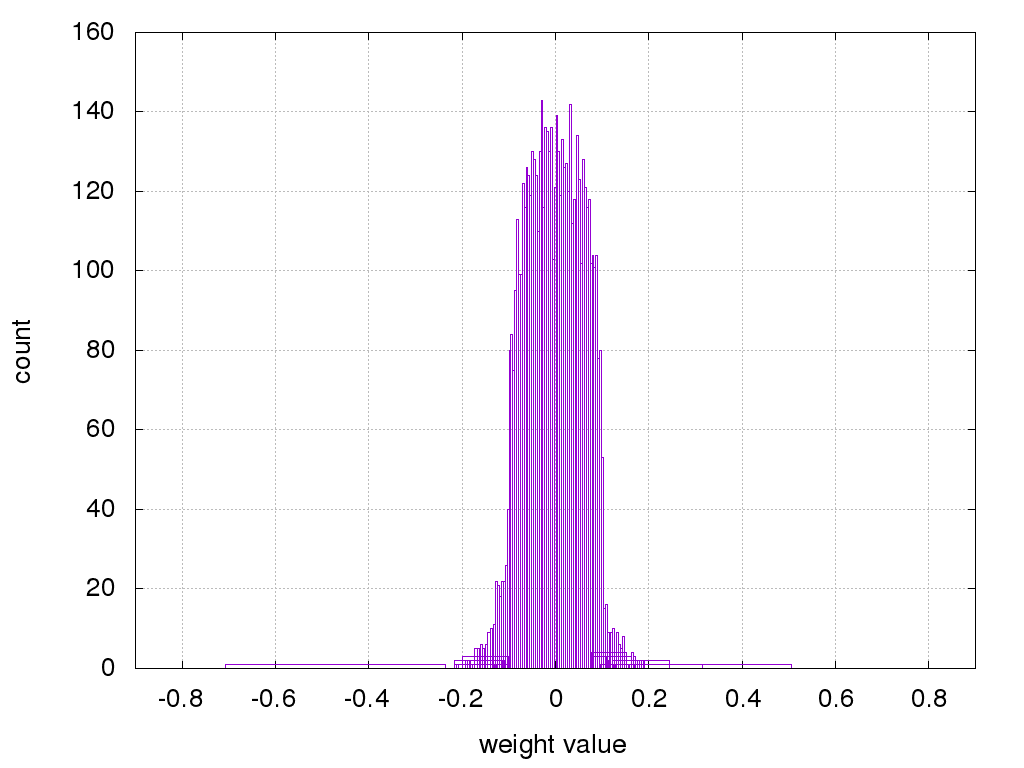
\includegraphics[scale=0.15]{../../results/rl_arcade/fnn_trained_5/supervised/layer_1_histogram.png}
  \captionof*{figure}{\tiny FNN no sparse weights histogram}
  \label{img:FNN no sparse weights histogram}
\end{minipage}
\end{figure}

\begin{figure}[!htb]
\centering
\begin{minipage}{.5\textwidth}
  \centering
  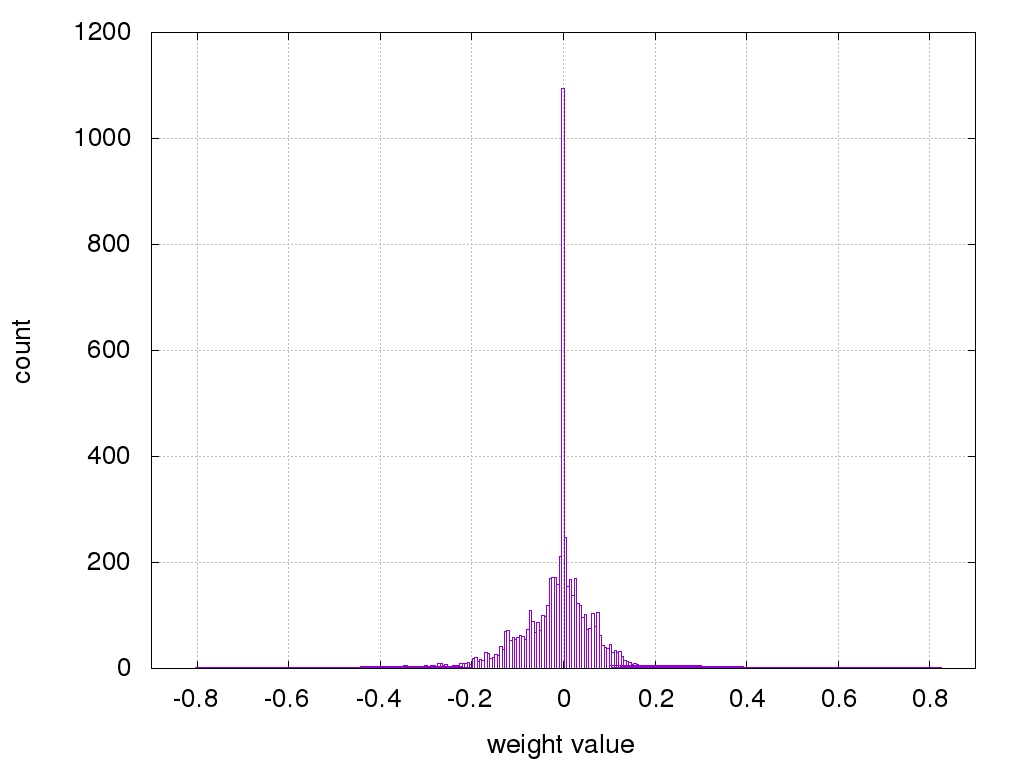
\includegraphics[scale=0.15]{../../results/rl_arcade/hnn_trained_0/supervised/layer_1_histogram.png}
  \captionof*{figure}{\tiny AE+FNN sparse weights histogram}
  \label{img:AE+FNN sparse weights histogram}
\end{minipage}%
\begin{minipage}{.5\textwidth}
  \centering
  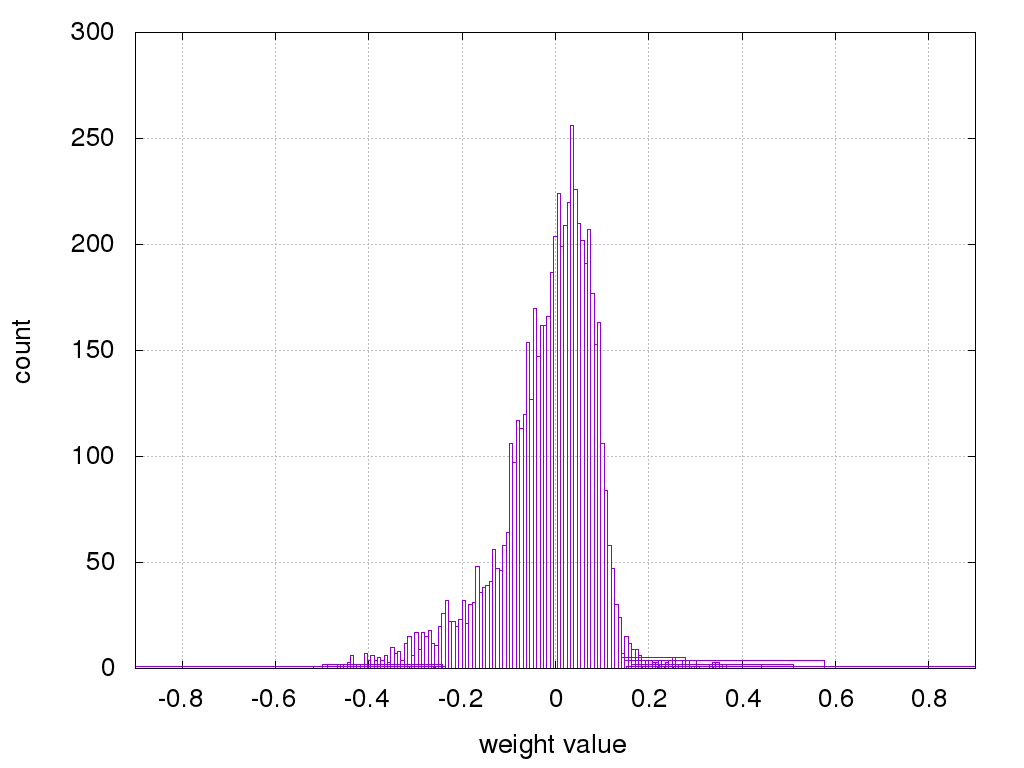
\includegraphics[scale=0.15]{../../results/rl_arcade/hnn_trained_5/supervised/layer_1_histogram.png}
  \captionof*{figure}{\tiny AE+FNN no sparse weights histogram}
  \label{img:AE+FNN no sparse weights histogram}
\end{minipage}
\end{figure}

\end{frame}



\begin{frame}{\bf Sparsity results}


\begin{figure}[htbp]
  \centering
  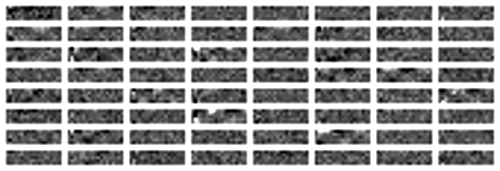
\includegraphics[scale=0.4]{../../diagrams/layer_1_fnn_sparse.png}
  \caption*{FNN sparse weights visualisation}
  \label{img:FNN sparse weights visualisation}
\end{figure}

\begin{figure}[htbp]
  \centering
  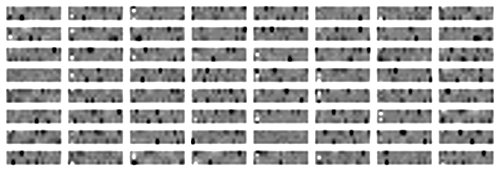
\includegraphics[scale=0.4]{../../diagrams/layer_1_hnn_sparse.png}
  \caption*{AE+FNN sparse weights visualisation}
  \label{img:AE+FNN sparse weights visualisation}
\end{figure}

\end{frame}








\begin{frame}{\bf Score results}


\begin{figure}[!htb]
\centering
\begin{minipage}{.5\textwidth}
  \centering
  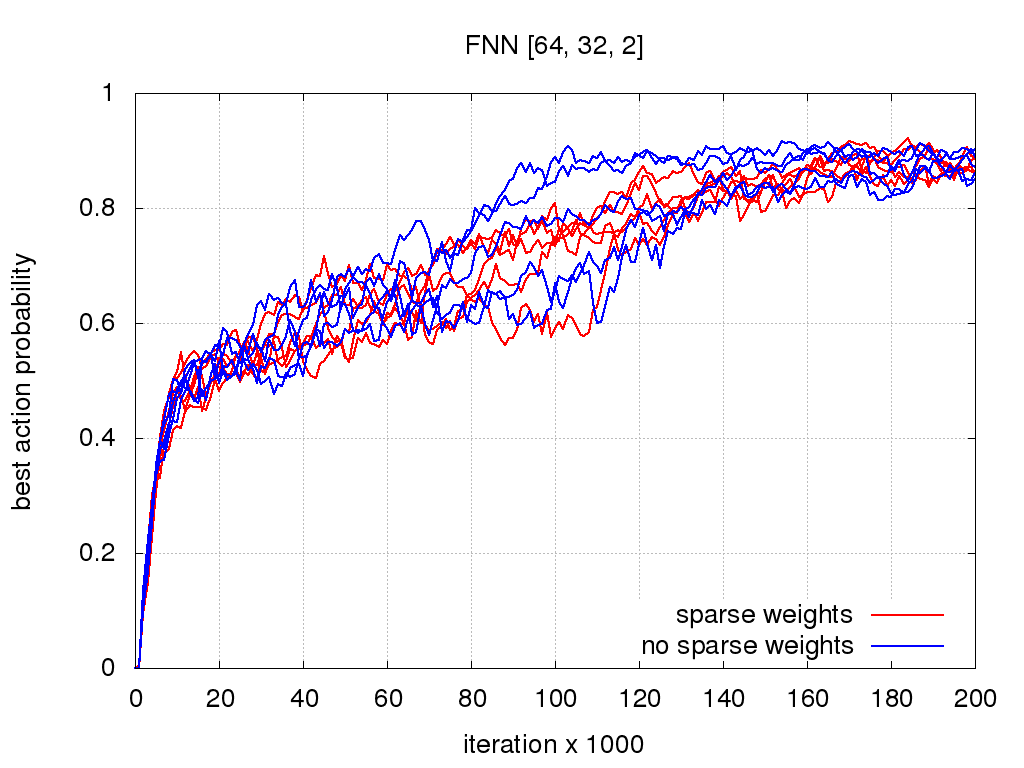
\includegraphics[scale=0.15]{../../results/rl_arcade/fnn_progress/training_progress.png}
  \captionof*{figure}{\tiny FNN progress comparison}
  \label{img:FNN progress comparison}
\end{minipage}%
\begin{minipage}{.5\textwidth}
  \centering
  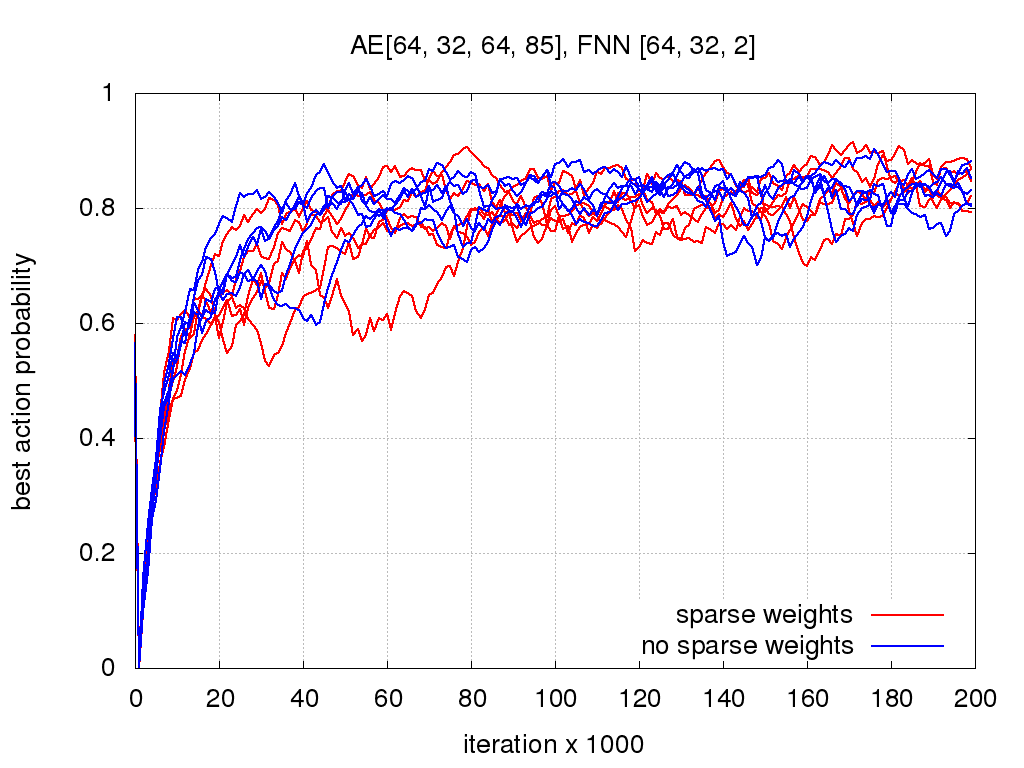
\includegraphics[scale=0.15]{../../results/rl_arcade/hnn_progress/training_progress.png}
  \captionof*{figure}{\tiny AE+FNN progress comparison}
  \label{img:AE+FNN progress comparison}
\end{minipage}
\end{figure}


\begin{figure}[!htb]
\centering
\begin{minipage}{.5\textwidth}
  \centering
  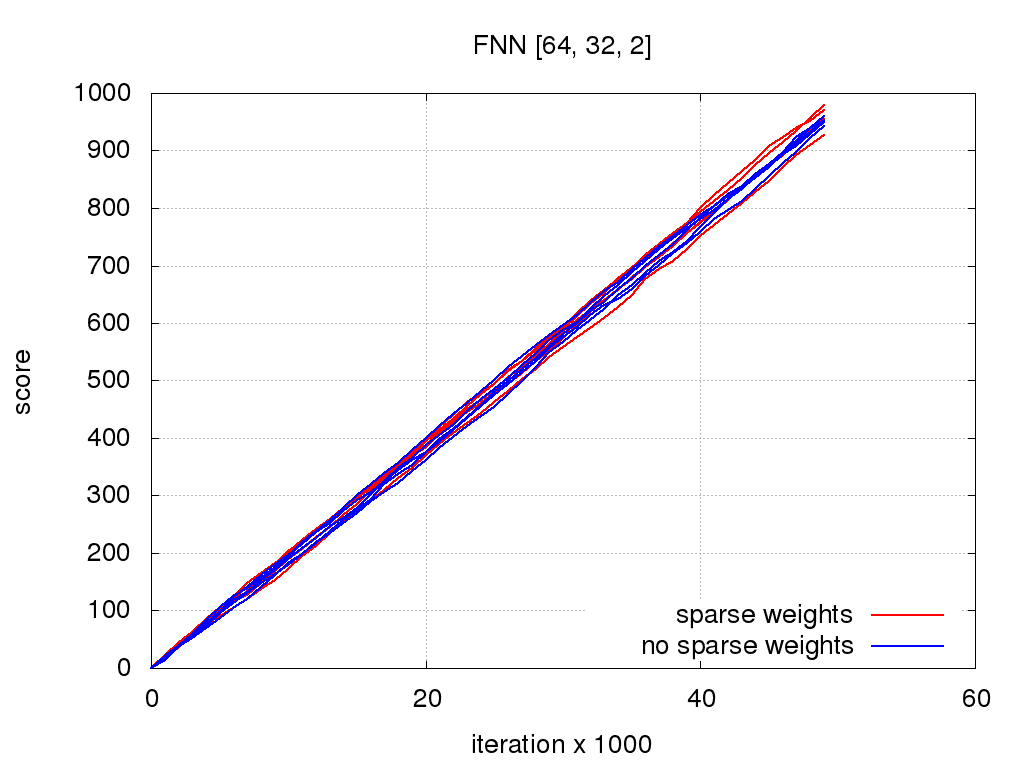
\includegraphics[scale=0.15]{../../results/rl_arcade/fnn_progress/testing_score.png}
  \captionof*{figure}{\tiny FNN score}
  \label{img:FNN score}
\end{minipage}%
\begin{minipage}{.5\textwidth}
  \centering
  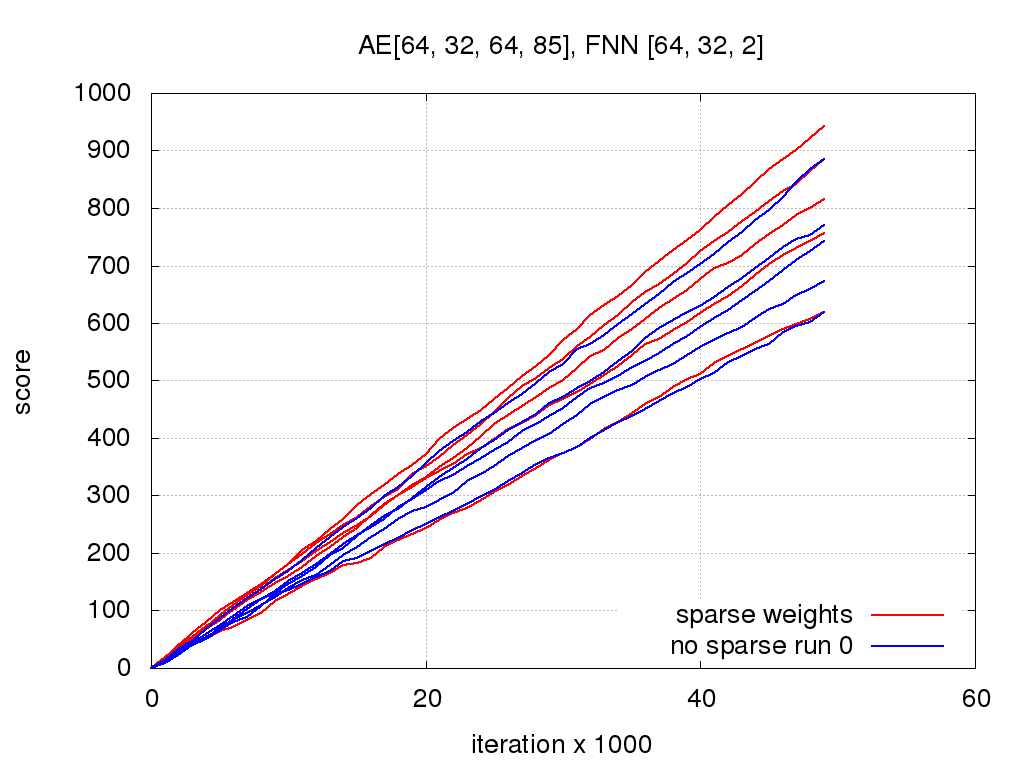
\includegraphics[scale=0.15]{../../results/rl_arcade/hnn_progress/testing_score.png}
  \captionof*{figure}{\tiny AE+FNN score}
  \label{img:AE+FNN score}
\end{minipage}
\end{figure}


\end{frame}


\begin{frame}{\bf Results}


\begin{figure}[!h]
  \centering
  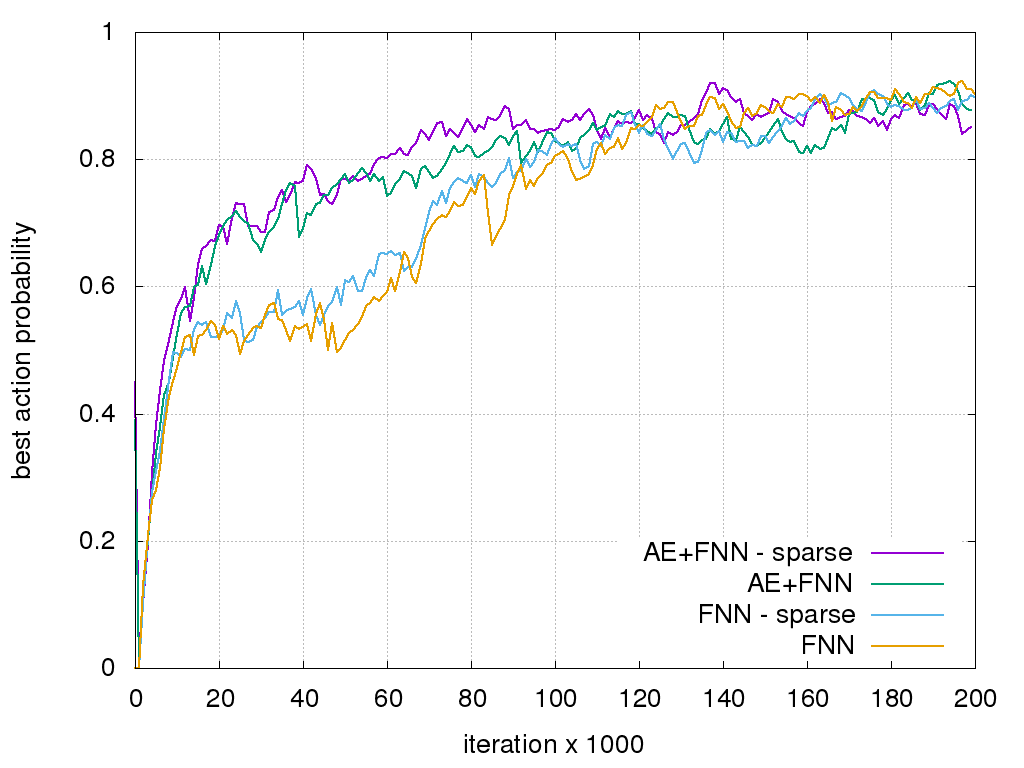
\includegraphics[scale=0.25]{../../results/rl_arcade/training_progress.png}
  \caption*{Training progress comparison}
  \label{img:Training progress comparison}
\end{figure}

{
\tiny
\begin{table}[]
\centering
\label{tab:summary_results}
\begin{tabular}{|l|c|c|c|c|}
\hline
                         & \multicolumn{1}{l|}{average score} & \multicolumn{1}{l|}{best score} & \multicolumn{1}{l|}{worst score} & \multicolumn{1}{l|}{average best action probability {[}\%{]}} \\ \hline
FNN sparse weights       & 960.58                             & 994.97                          & 922.64                           & 95.32                                                         \\ \hline
FNN nosparse weights     & 945.04                             & 995.64                          & 878.31                           & 93.29                                                         \\ \hline
AE+FNN sparse weights    & 914.5                              & 947.64                          & 875.31                           & 93.4                                                          \\ \hline
AE+FNN no sparse weights & 908.58                             & 954.31                          & 780.32                           & 93.12                                                         \\ \hline
\end{tabular}
\end{table}
}

\end{frame}












\begin{frame}{\bf Snake game experiment}


\begin{figure}[htbp]
  \centering
  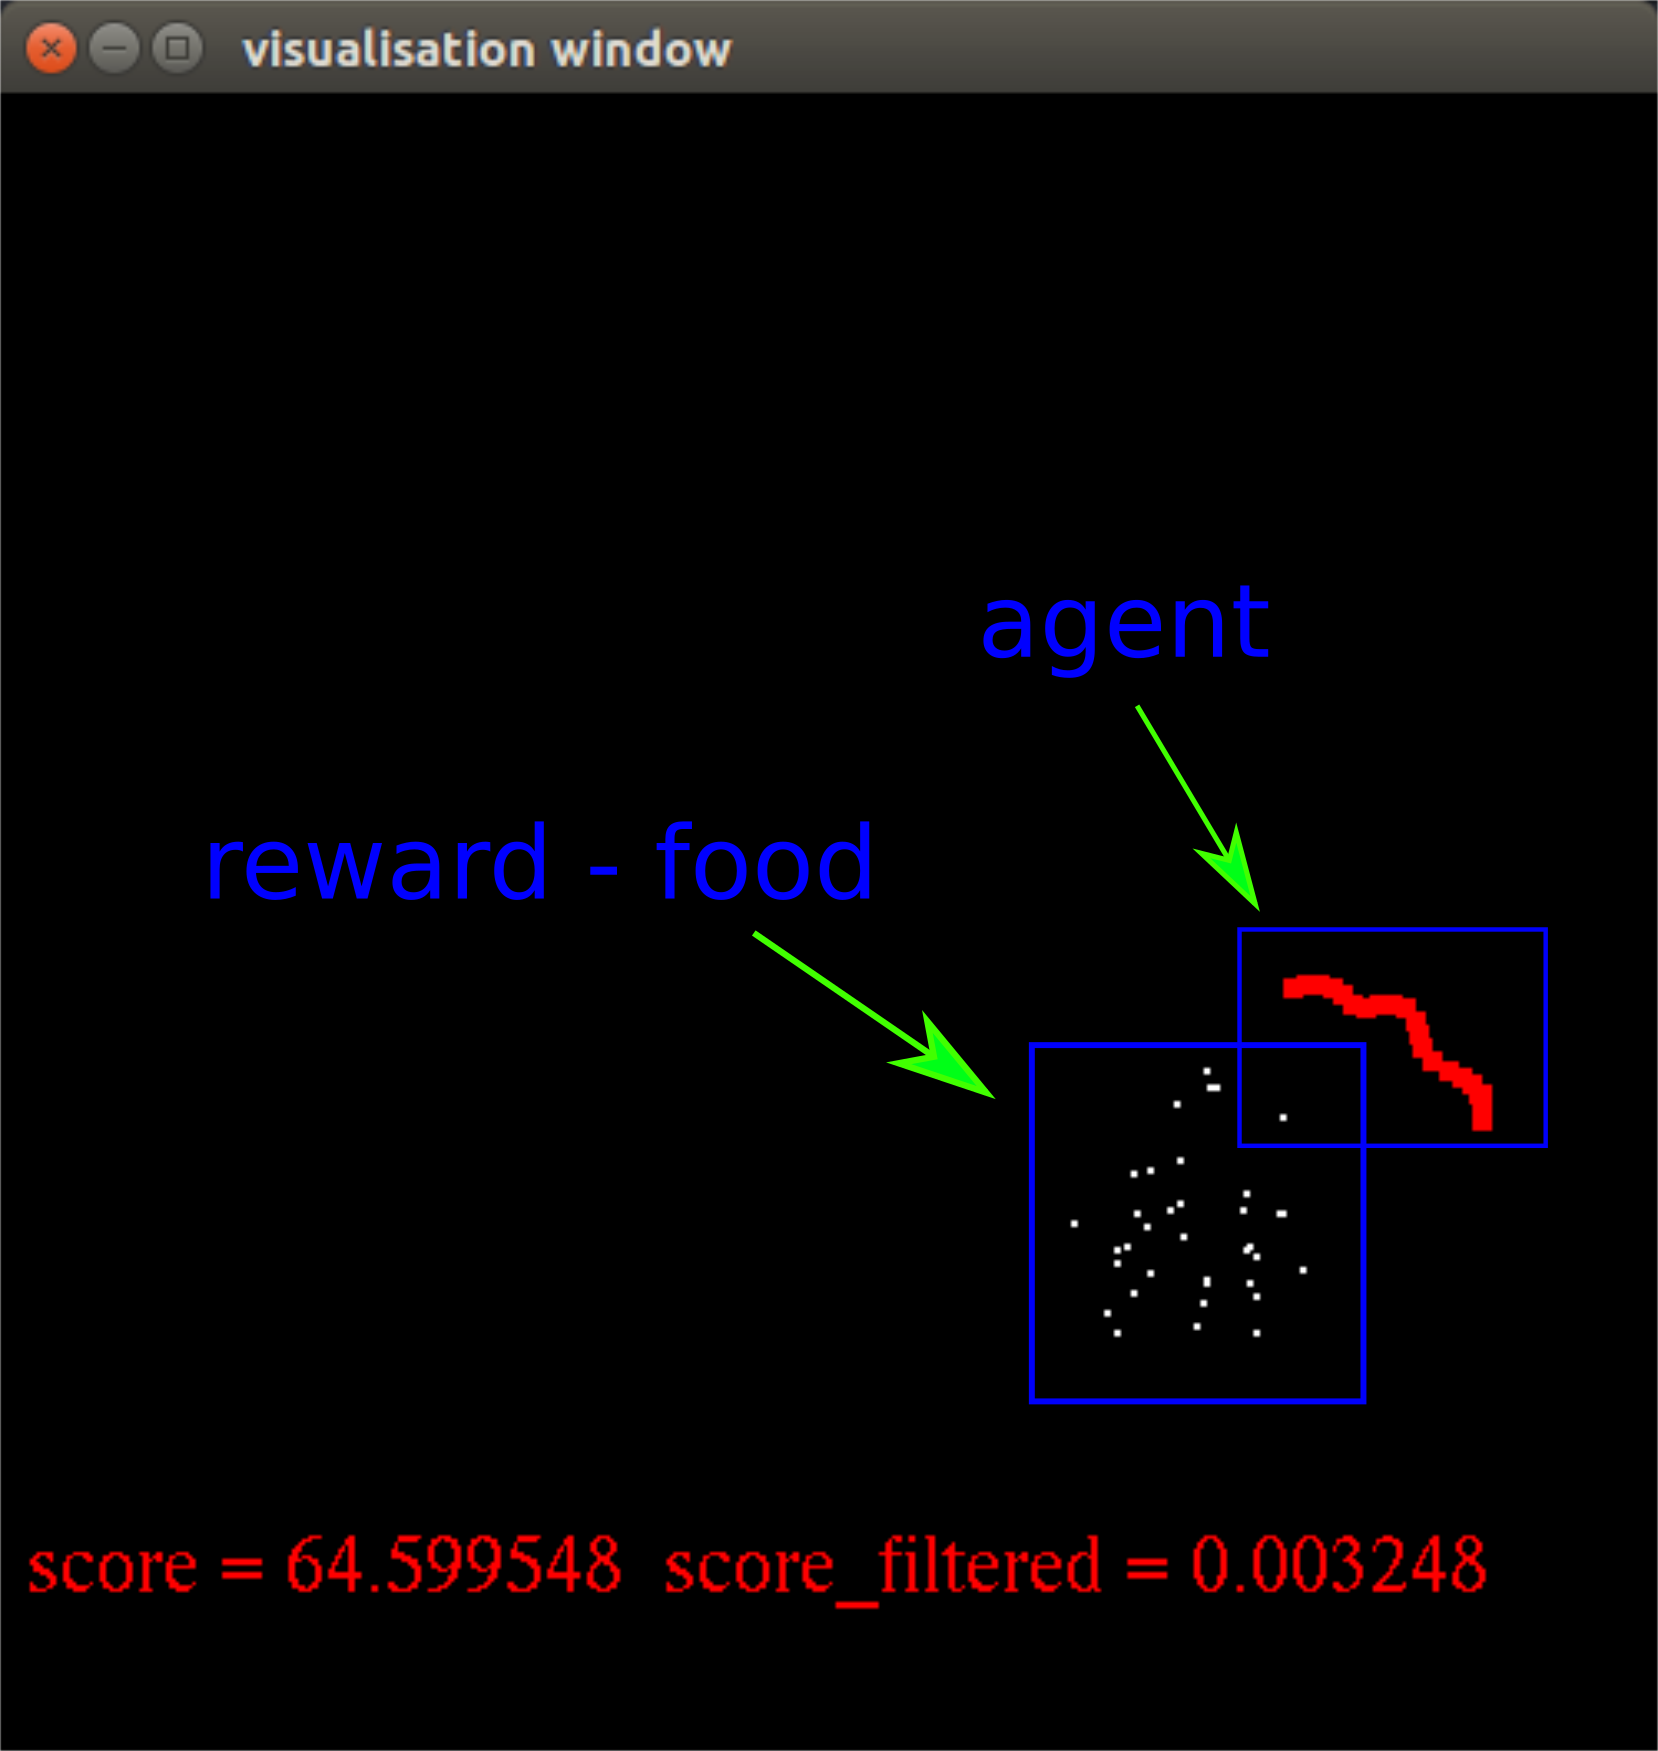
\includegraphics[scale=0.15]{../../diagrams/worms_rl_game_desc.png}
\end{figure}

\begin{figure}[!htb]
\centering
\begin{minipage}{.5\textwidth}
  \centering
  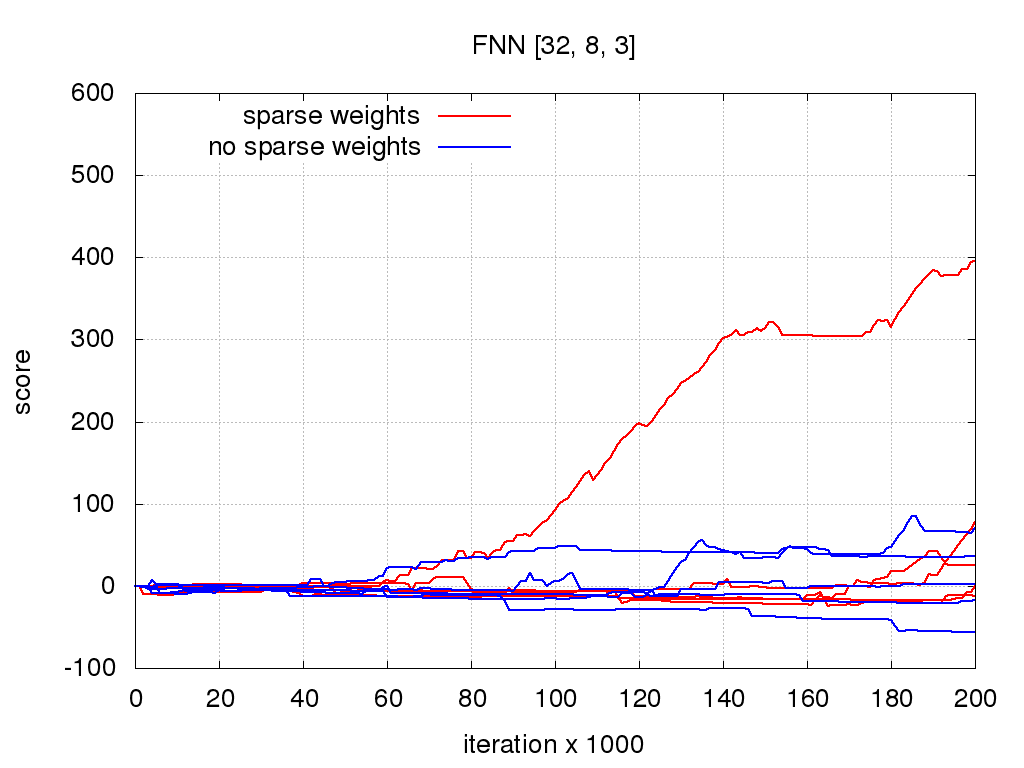
\includegraphics[scale=0.17]{../../results/rl_worms/fnn_progress/training_progress.png}
  \captionof*{figure}{FNN score progress comparison}
  \label{img:worms FNN score progress comparison}
\end{minipage}%
\begin{minipage}{.5\textwidth}
  \centering
  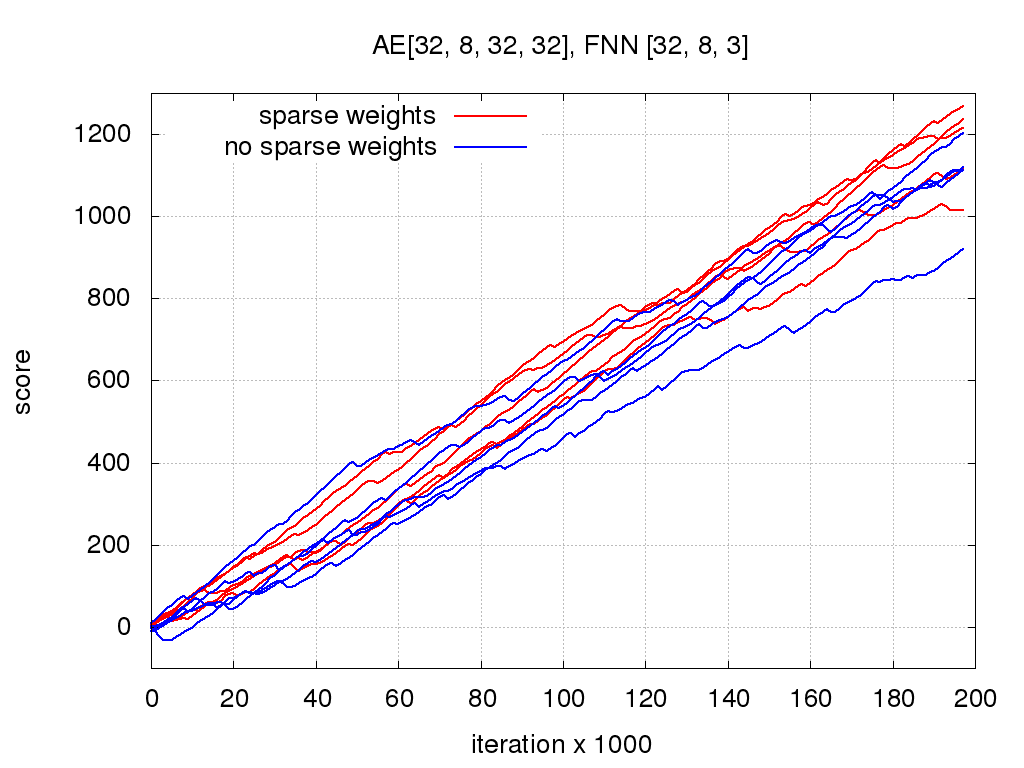
\includegraphics[scale=0.17]{../../results/rl_worms/hnn_progress/training_progress.png}
  \captionof*{figure}{AE+FNN score progress comparison}
  \label{img:worms AE+FNN score progress comparison}
\end{minipage}
\end{figure}

\end{frame}



\begin{frame}{\bf Snake game experiment}


\begin{figure}[!h]
  \centering
  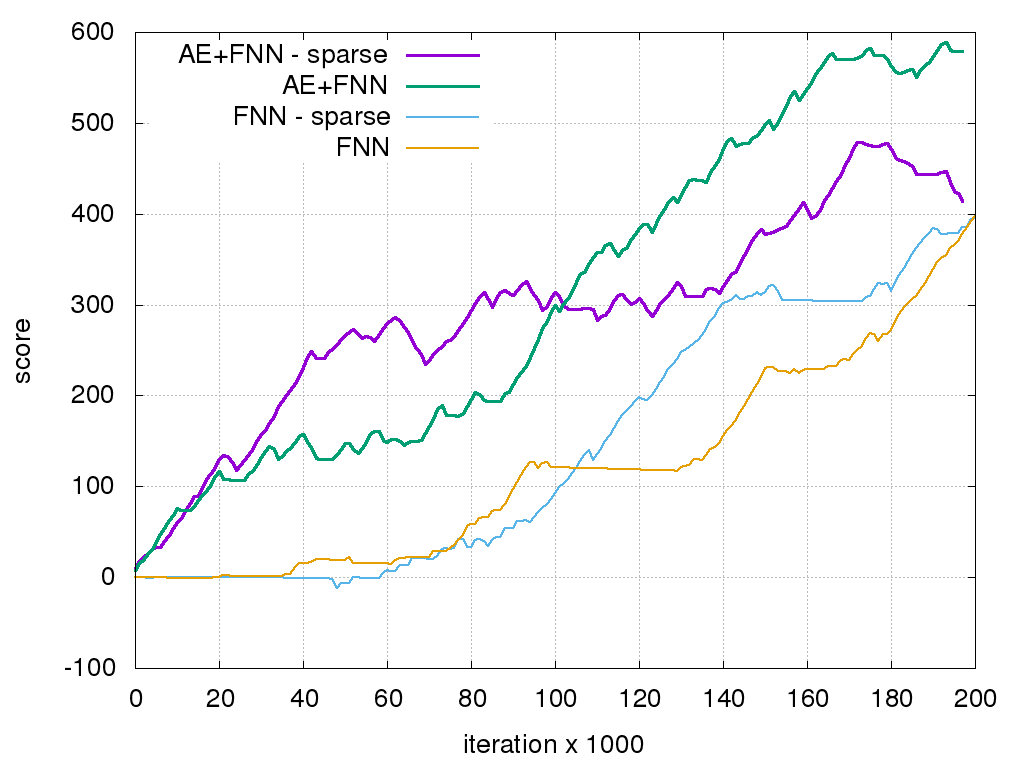
\includegraphics[scale=0.3]{../../results/rl_worms/training_progress.png}
  \caption*{Training worms score progress for best networks}
  \label{img:Training worms score progress for best networks}
\end{figure}

\end{frame}


%-------------------------------------------------------------------------------------
\begin{frame}{\bf Q\&A}

\begin{figure}[ht]
\begin{center}
\begin{minipage}{0.8\linewidth}
\begin{center}
 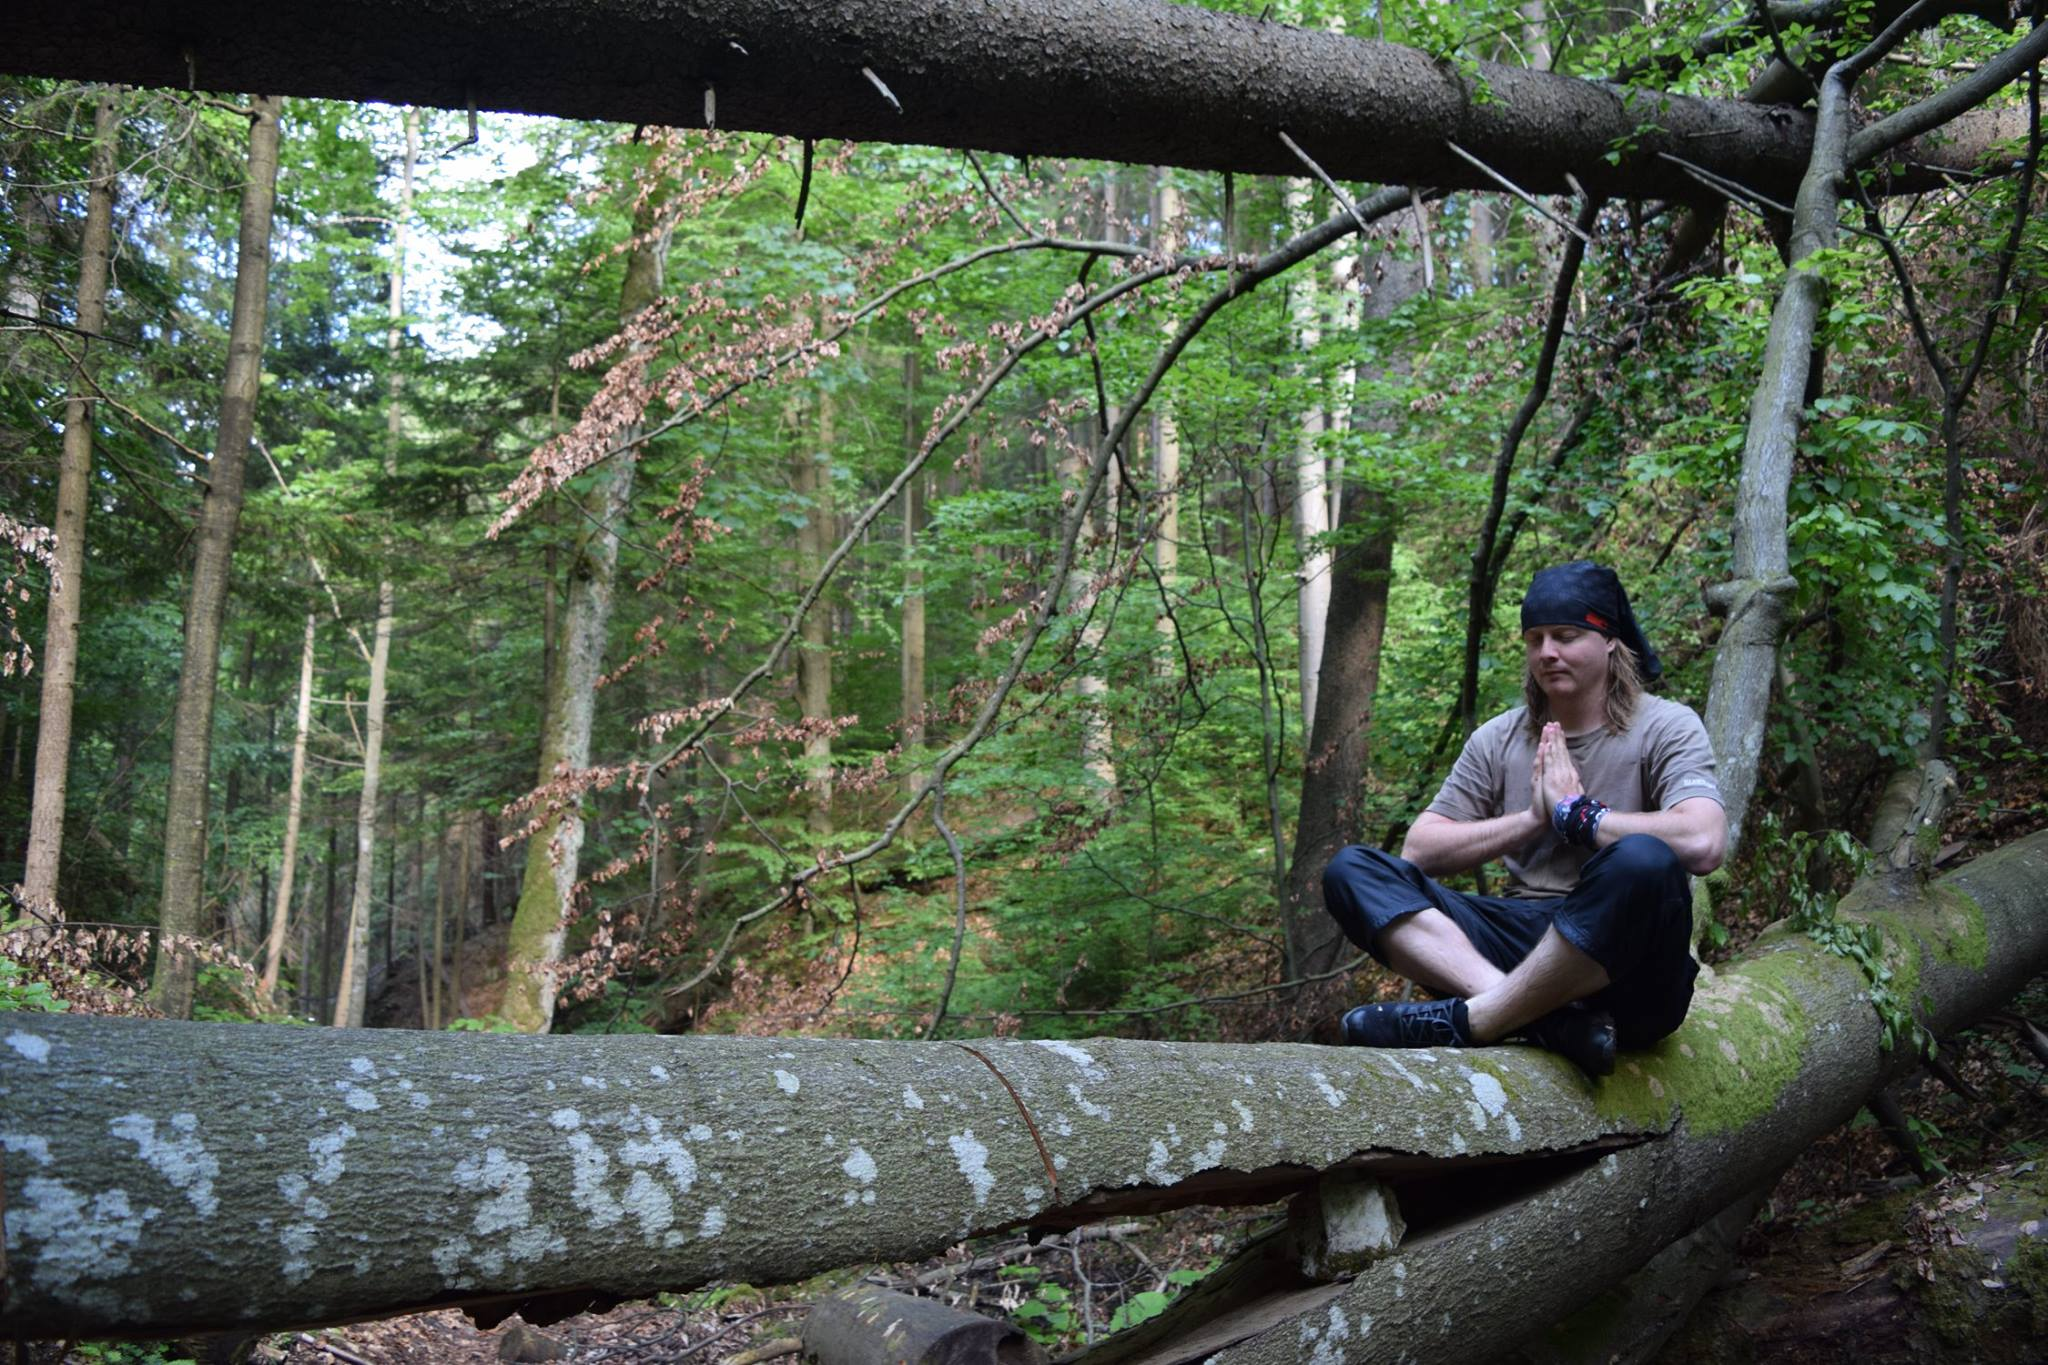
\includegraphics[width=1.0\textwidth]{../../pictures/me.jpg}
\end{center}
\end{minipage}
\end{center}
\end{figure}

\url{https://github.com/michalnand/robotics}
\url{https://github.com/michalnand/machine\_learning}

\centerline{michal.nand@gmail.com}

\end{frame}

\end{document}
